% ***************************************************************************************************
%
%	Szablon pracy magisterskiej dla Politechniki Wrocławskiej w wersji dwustronnej.
%	Autor:	Tomasz Strzałka
%
% ***************************************************************************************************

% Styl dwustronny z domyślną wielkością czcionki 11pt oraz oddzieloną stroną tytułową (titlepage).
% Domyślnie rodziały rozpoczynają się na stronie prawej (openright).
\documentclass[a4paper,11pt]{book}

% ***************************************************************************************************
% Ustawienia języka
% ***************************************************************************************************

% Podstawowe ustawienia języka, według którego formatowany będzie dokument
\usepackage[polish]{babel}

% Pakiet babel dla polskiego języka powoduje konflikt z pakietem amssymb.
% Polecenie '\lll' definiują oba pakiety - porządana jest druga definicja.
\let\lll\undefined

% W przypadku wielojęzykowości ustawia główny język dokumentu
\selectlanguage{polish}
\usepackage[fixlanguage]{babelbib}

% Kodowanie dokumentu
\usepackage[utf8]{inputenc}

% Dowolny rozmiar czcionek, kodowanie znaków
\usepackage{lmodern}

% Polskie wcięcia akapitów
\usepackage{indentfirst}

% Polskie łamanie wyrazów
\usepackage[plmath]{polski}

% Przecinek w wyrażeniach matematycznych zamiast kropki
\usepackage{icomma}

% Polskie formatowanie typograficzne
\frenchspacing

% Zapewnia liczne usprawnienia wyświetlania i organizacji matematycznych formuł. 
\usepackage{amsmath}

% Wprowadza rozszerzony zestaw symboli m.in. \leadsto
\usepackage{amssymb}

% Dodatkowa, ,,kręcona'' czcionka matematyczna
\usepackage{mathrsfs}

% Dodatkowe wsparcie dla środowiska mathbb, które nie wspiera domyślnie cyfr (\mathbb{})
\usepackage{bbold}

% Dodaje kolory
\usepackage[table]{xcolor}


% Fixes/improves amsmath
\usepackage{mathtools}


% ***************************************************************************************************
% Kolory  
% ***************************************************************************************************

% Umożliwia kolorowanie poszczególnych komórek tabeli
\usepackage[table]{xcolor}% http://ctan.org/pkg/

% Umożliwia łatwą zmianę koloru linii w tabeli
\usepackage{tabu}

% Definicje kolorów
\definecolor{lred}{HTML}{FFB0B0}
\definecolor{lgray}{HTML}{9F9F9F}
\definecolor{dgray}{HTML}{5F5F5F}
\definecolor{sgreen}{HTML}{006122}
% lgray				-	nazwa nowo zdefiniowanego koloru
% HTML				-	model kolorów
% CCCCCC			-	wartość koloru zgodna z modelem

% ***************************************************************************************************
% Algorytmy 
% ***************************************************************************************************

% Udostępnia środowisko do konstruowania pseudokodów
\usepackage[Pseudokod]{algorithm}
\usepackage{algpseudocode}
% ruled	- poziome kreski na początku i końcu algorytmu, podpis na górze oddzielony również kreską poziomą
% vlined - pionowe kreski łączące początek polecenia z jego końcem
% linesnumbered	- numerowanie kolejnych wierszy algorytmu
% longend - długie końcówki np. ifend, forend itd.
% algochapter - numeracja z rozdziałami

% Zamiana nazwy środowiska z domyślnej "Algorithm X" na "Pseudokod X"
\newenvironment{pseudokod}[1][!htb]{
	\renewcommand{\algorithmcfname}{Pseudokod}
	\begin{algorithm}[#1]%
	}{
\end{algorithm}
}

\makeatletter 
\renewcommand\thealgorithm{\thechapter.\arabic{algorithm}} 
\@addtoreset{algorithm}{chapter} 
\makeatother


\algdef{SE}[CLASS]{Class}{EndClass}[1]{\textbf{class} \textsc{#1}}{\textbf{end class}}
\algdef{SE}[CONSTRUCTOR]{Constructor}{EndConstructor}[1]{\textbf{constructor}\ifthenelse{\equal{#1}{}}{}{(#1)}}{\textbf{end constructor}}

% Zmiana rozmiaru komentarzy
%\newcommand\algcomment[1]{
%	\footnotesize{#1}
%}

% Ustawienie zadanego stylu dla komentarzy
%\SetCommentSty{algcomment}

% Wyśrodkowana tylda
\usepackage{textcomp}%
\newcommand{\textapprox}{\raisebox{0.5ex}{\texttildelow}}

% Listowanie kodów źródłowych
\usepackage{listings} 
\renewcommand{\lstlistingname}{Kod źródłowy} % Polska nazwa listingu
\lstset{ 
    commentstyle=\color{dgray},
    keywordstyle=\color{blue},
    stringstyle=\color{sgreen},
    numbers=left
}

% Definicje pecjalnych znaków, które nie są obsługiwane w środowisku listing
\lstset{literate=
	{ż}{{\.{z}}}1	{ź}{{\'{z}}}1
	{ć}{{\'{c}}}1	{ń}{{\'{n}}}1
	{ą}{{\c a}}1	{ś}{{\'{s}}}1
	{ł}{{\l}}1		{ę}{{\c{e}}}1
	{ó}{{\'{o}}}1	{á}{{\'a}}1
	{é}{{\'e}}1		{í}{{\'i}}1
	{ó}{{\'o}}1		{ú}{{\'u}}1
	{ù}{{\`u}}1		{Á}{{\'A}}1
	{É}{{\'E}}1		{Í}{{\'I}}1
	{Ó}{{\'O}}1		{Ú}{{\'U}}1
	{à}{{\`a}}1		{è}{{\'e}}1
	{ì}{{\`i}}1		{ò}{{\`o}}1
	{ò}{{\`o}}1		{À}{{\`A}}1
	{È}{{\'E}}1		{Ì}{{\`I}}1
	{Ò}{{\`O}}1		{Ò}{{\`O}}1
	{ä}{{\"a}}1		{ë}{{\"e}}1
	{ï}{{\"i}}1		{ö}{{\"o}}1
	{ü}{{\"u}}1		{Ä}{{\"A}}1
	{Ë}{{\"E}}1		{Ï}{{\"I}}1
	{Ö}{{\"O}}1		{Ü}{{\"U}}1
	{â}{{\^a}}1		{ê}{{\^e}}1
	{î}{{\^i}}1		{ô}{{\^o}}1
	{û}{{\^u}}1		{Â}{{\^A}}1
	{Ê}{{\^E}}1		{Î}{{\^I}}1
	{Ô}{{\^O}}1		{Û}{{\^U}}1
	{œ}{{\oe}}1		{Œ}{{\OE}}1
	{æ}{{\ae}}1		{Æ}{{\AE}}1
	{ß}{{\ss}}1		{ç}{{\c c}}1
	{Ç}{{\c C}}1	{ø}{{\o}}1
	{å}{{\r a}}1	{Å}{{\r A}}1
	{€}{{\EUR}}1	{£}{{\pounds}}1
}

% ***************************************************************************************************
% Marginesy 
% ***************************************************************************************************

% Ustawienia rozmiarów stron i ich marginesów
\usepackage[headheight=18pt, top=25mm, bottom=25mm, left=25mm, right=25mm]{geometry}
% headheight		-	wysokość tytułów
% top				-	margines górny
% bottom			-	margines dolny
% left				-	margines lewy
% right				-	margines prawy

% Usunięcie górnego marginesu dla środowisk
\makeatletter
\setlength\@fptop{0\p@}	
\makeatother

% ***************************************************************************************************
% Styl 
% ***************************************************************************************************

% Definiuje środowisko 'titlingpage', które zapewnia pełną kontrolę nad układem strony tytułowej.
\usepackage{titling}


% Umożliwia modyfikowanie stylu spisu treści
\usepackage{tocloft}	

\tocloftpagestyle{tableOfContentStyle}

% Definiowanie własnych stylów nagłówków i/lub stopek
\usepackage{fancyhdr}

% Domyślny styl dla pracy 
\fancypagestyle{custom}{
	\fancyhf{}									% wyczyść stopki i nagłówki
	\fancyhead[RO]{								% Prawy, nieparzysty nagłówek
		\hrulefill \hspace{16pt} \large Rozdział \thechapter
		\put(-472.1, 12.1){%
			\makebox(0,0)[l]{%
				
\includegraphics[width=0.05\textwidth]{pwr-logo}
			}
		}
		\put(-443,5.5){%
			\makebox(0,0)[l]{%
				\small Politechnika Wrocławska
			}
		}
	}
	\fancyhead[LE]{								% Lewy, parzysty nagłówek
		\large Rozdział \thechapter \hspace{16pt} \hrulefill 
		\put(-22, 12.1){%
			\makebox(0,0)[l]{%
				
\includegraphics[width=0.05\textwidth]{wit-logo}
			}
		}
		\put(-210,5.5){%
			\makebox(0,0)[l]{%
				\small Wydział Informatyki i Telekomunikacji
			}
		}
	}
	\fancyfoot[LE,RO]{							% Stopki
		\thepage
	}
	\renewcommand{\headrulewidth}{0pt}			% Grubość linii w nagłówku
	\renewcommand{\footrulewidth}{0.2pt}		% Grubość linii w stopce
}


% Domyślny styl dla bibliografii
\fancypagestyle{bibliographyStyle}{
	\fancyhf{}									% wyczyść stopki i nagłówki
	\fancyhead[RO]{								% Prawy, nieparzysty nagłówek
		\hrulefill \hspace{16pt} \large Dodatek \thechapter
		\put(-472.1, 12.1){%
			\makebox(0,0)[l]{%
				
\includegraphics[width=0.05\textwidth]{pwr-logo}
			}
		}
		\put(-443,5.5){%
			\makebox(0,0)[l]{%
				\small Politechnika Wrocławska
			}
		}
	}
	\fancyhead[LE]{								% Lewy, parzysty nagłówek
		\large Bibliografia \hspace{16pt} \hrulefill 
		\put(-22, 12.1){%
			\makebox(0,0)[l]{%
				
\includegraphics[width=0.05\textwidth]{wit-logo}
			}
		}
		\put(-210,5.5){%
			\makebox(0,0)[l]{%
				\small Wydział Informatyki i Telekomunikacji
			}
		}
	}
	\fancyfoot[LE,RO]{							% Stopki
		\thepage
	}
	\renewcommand{\headrulewidth}{0pt}			% Grubość linii w nagłówku
	\renewcommand{\footrulewidth}{0.2pt}		% Grubość linii w stopce
}

% Domyślny styl dla dodatków
\fancypagestyle{appendixStyle}{
	\fancyhf{}									% wyczyść stopki i nagłówki
	\fancyhead[RO]{								% Prawy, nieparzysty nagłówek
		\hrulefill \hspace{16pt} \large Dodatek \thechapter
		\put(-472.1, 12.1){%
			\makebox(0,0)[l]{%
				
\includegraphics[width=0.05\textwidth]{pwr-logo}
			}
		}
		\put(-443,5.5){%
			\makebox(0,0)[l]{%
				\small Politechnika Wrocławska
			}
		}
	}
	\fancyhead[LE]{								% Lewy, parzysty nagłówek
		\large Dodatek \thechapter \hspace{16pt} \hrulefill 
		\put(-22, 12.1){%
			\makebox(0,0)[l]{%
				
\includegraphics[width=0.05\textwidth]{wit-logo}
			}
		}
		\put(-210,5.5){%
			\makebox(0,0)[l]{%
				\small Wydział Informatyki i Telekomunikacji
			}
		}
	}
	\fancyfoot[LE,RO]{							% Stopki
		\thepage
	}
	\renewcommand{\headrulewidth}{0pt}			% Grubość linii w nagłówku
	\renewcommand{\footrulewidth}{0.2pt}		% Grubość linii w stopce
}

% Osobny styl dla stron zaczynających rozdział/spis treści itd. (domyślnie formatowane jako "plain")
\fancypagestyle{chapterBeginStyle}{
	\fancyhf{}%
	\fancyfoot[LE,RO]{
		\thepage
	}
	\renewcommand{\headrulewidth}{0pt}
	\renewcommand{\footrulewidth}{0.2pt}
}

% Styl dla pozostałych stron spisu treści
\fancypagestyle{tableOfContentStyle}{
	\fancyhf{}%
	\fancyfoot[LE,RO]{
		\thepage
	}
	\renewcommand{\headrulewidth}{0pt}
	\renewcommand{\footrulewidth}{0.2pt}
}

% Formatowanie tytułów rozdziałów i/lub sekcji
\usepackage{titlesec}

% Formatowanie tytułów rozdziałów
\titleformat{\chapter}[hang]					% kształt
{
	\vspace{-10ex}
	\Huge
	\bfseries
}												% formatowanie tekstu modyfikowanego elementu
{}												% etykieta występująca przed tekstem modyfikowanego elementu, niewidoczna w spisie treści
{
	10pt
}												% odstęp formatowanego tytułu od lewego marginesu/etykiety
{
	\Huge
	\bfseries
}												% formatowanie elementów przed modyfikowanym tytułem
[
\vspace{2ex}
%\rule{\textwidth}{0.4pt}
%\vspace{-4ex}
]												% dodatkowe formatowanie stosowane poniżej modyfikowanego tytułu


% Formatowanie tytułów sekcji
\titleformat{\section}[hang]					% kształt
{
	\vspace{2ex}
%	\titlerule\vspace{1ex}
	\Large\bfseries
}												% formatowanie tekstu modyfikowanego elementu
{
	\thesection									% etykieta występująca przed tekstem modyfikowanego elementu, niewidoczna w spisie treści
}
{
	0pt
}												% odstęp formatowanego tytułu od lewego marginesu/etykiety
{
	\Large
	\bfseries
}												% formatowanie elementów przed modyfikowanym tytułem

% ***************************************************************************************************
% Linki
% ***************************************************************************************************

% Umożliwia wstawianie hiperłączy do dokumentu
\usepackage{hyperref}							% Aktywuje linki

\hypersetup{
	colorlinks	=	true,					% Koloruje tekst zamiast tworzyć ramki.
	linkcolor		=	black,					% Kolory: referencji,
    citecolor		=	dgray,					% cytowań,
	urlcolor		=	dgray					% hiperlinków.
}

% Do stworzenia hiperłączy zostanie użyta ta sama (same) czcionka co dla reszty dokumentu
\urlstyle{same}
\renewcommand\UrlFont\itshape



% ***************************************************************************************************
% Linki
% ***************************************************************************************************

% Umożliwia zdefiniowanie własnego stylu wyliczeniowego
\usepackage{enumitem}

% Nowa lista numerowana z trzema poziomami
\newlist{myitemize}{itemize}{3}

% Definicja wyglądu znacznika pierwszego poziomu
\setlist[myitemize,1]{
	label		=	\textbullet,
	leftmargin	=	4mm}

% Definicja wyglądu znacznika drugiego poziomu
\setlist[myitemize,2]{
	label		=	$\diamond$,
	leftmargin	=	8mm}

% Definicja wyglądu znacznika trzeciego poziomu
\setlist[myitemize,3]{
	label		=	$\diamond$,
	leftmargin	=	12mm
}

% ***************************************************************************************************
% Inne pakiety
% ***************************************************************************************************

% Dołączanie rysunków
\usepackage{graphicx}

% Figury i przypisy
\usepackage{caption}
\usepackage{subcaption}

% Umożliwia tworzenie przypisów wewnątrz środowisk
\usepackage{footnote}

% Umożliwia tworzenie struktur katalogów
\usepackage{dirtree}

% Rozciąganie komórek tabeli na wiele wierszy
\usepackage{multirow}

% Precyzyjne obliczenia szerokości/wysokości dowolnego fragmentu wygenerowanego przez LaTeX
\usepackage{calc}

% ***************************************************************************************************
% Matematyczne skróty
% ***************************************************************************************************

% Skrócony symbol liczb rzeczywistych
\newcommand{\RR}{\mathbb{R}}

% Skrócony symbol liczb naturalnych
\newcommand{\NN}{\mathbb{N}}

% Skrócony symbol liczb wymiernych
\newcommand{\QQ}{\mathbb{Q}}

% Skrócony symbol liczb całkowitych
\newcommand{\ZZ}{\mathbb{Z}}

% Skrócony symbol logicznej implikacji
\newcommand{\IMP}{\rightarrow}

% Skrócony symbol  logicznej równoważności
\newcommand{\IFF}{\leftrightarrow}

% ***************************************************************************************************
% Środowiska
% ***************************************************************************************************

% Środowisko do twierdzeń
\newtheorem{theorem}{Twierdzenie}[chapter]

% Środowisko do lematów
\newtheorem{lemma}{Lemat}[chapter]

% Środowisko do przykładów
\newtheorem{example}{Przykład}[chapter]

% Środowisko do wniosków
\newtheorem{corollary}{Wniosek}[chapter]

% Środowisko do definicji
\newtheorem{definition}{Definicja}[chapter]

% Środowisko do dowodów
\newenvironment{proof}{
	\par\noindent \textbf{Dowód.}
}{
\begin{flushright}
	\vspace*{-6mm}\mbox{$\blacklozenge$}
\end{flushright}
}

% Środowisko do uwag
\newenvironment{remark}{
	\bigskip \par\noindent \small \textbf{Uwaga.}
}{
\begin{small}
	\vspace*{4mm}
\end{small}
}
%ALD - nowe środowisko do streszczenia i abstractu
\newenvironment{streszczenie}{
	\par\noindent {\large \textbf{Streszczenie}\\[14pt]\indent}
}{}
\newenvironment{abstract}{
	\par\noindent {\large \textbf{Abstract}\\[14pt]\indent}
}{}

% ***************************************************************************************************
% Słownik
% ***************************************************************************************************

% Prawidłowe dzielenie wyrazów
\hyphenation{wszy-stkich ko-lu-mnę każ-da od-leg-łość
	dzie-dzi-ny dzie-dzi-na rów-nych rów-ny
	pole-ga zmie-nna pa-ra-met-rów wzo-rem po-cho-dzi
	o-trzy-ma wte-dy wa-run-ko-wych lo-gicz-nie
	skreś-la-na skreś-la-ną cał-ko-wi-tych wzo-rów po-rzą-dek po-rząd-kiem
	przy-kład pod-zbio-rów po-mię-dzy re-pre-zen-to-wa-ne
	rów-no-waż-ne bi-blio-te-kach wy-pro-wa-dza ma-te-ria-łów
	prze-ka-za-nym skoń-czo-nym moż-esz na-tu-ral-na cią-gu tab-li-cy
	prze-ka-za-nej od-po-wied-nio}

% ***************************************************************************************************
% Dokument
% ***************************************************************************************************
\frontmatter

\begin{document}

	\begin{titlingpage}
		\vspace*{\fill}
		\begin{center}
			\begin{picture}(300,510)
				\put(11,520){\makebox(0,0)[l]{\large \textsc{Wydział Informatyki i Telekomunikacji}}}
				\put(11,500){\makebox(0,0)[l]{\large \textsc{Politechnika Wrocławska}}}
% Tytuł pracy
				\put(20,320){\Huge \textsc{Generowanie liczb losowych}}
				\put(20,280){\Huge \textsc{w oparciu o czas dostępu}}
				\put(20,240){\Huge \textsc{do zasobów sieciowych}}
% Autor pracy
				\put(30,200){\makebox(0,0)[l]{\large \textsc{Marek Bauer}}}
				\put(30,180){\makebox(0,0)[l]{\large \textsc{Nr indeksu: 250076}}}

				\put(200,100){\makebox(0,0)[l]{\large Praca inżynierska napisana}}
				\put(200,80){\makebox(0,0)[l]{\large pod kierunkiem}}
% dane promotora
				\put(200,60){\makebox(0,0)[l]{\large dr. hab. Szymona Żeberskiego}}
				
				\put(115,-70){
\includegraphics[width=0.15\textwidth]{pwr}}
				\put(106,-80){\makebox(0,0)[bl]{\large \textsc{Wrocław 2021}}}
			\end{picture}
		\end{center}	
		\vspace*{\fill}
	\end{titlingpage}
	
    \cleardoublepage
	\begin{streszczenie}
Celem pracy jest stworzenie prostego generatora jednostajnych i niezależnych liczb losowych. Źródłem entropii dla niego będą czasy opóźnień, które powstają podczas przesyłania pakietów przez Internet. Zostaną zaprezentowane wyniki testów wydajności, jak i losowości tego podejścia. Losowość zostanie sprawdzona w oparciu o testy statystyczne zaproponowane w tej pracy, a wyniki niniejszego generatora porównane do trzech znanych na rynku rozwiązań różnej klasy.
\end{streszczenie}

	\vspace*{1cm}	
    \begin{abstract}
The purpose of this thesis is to create a simple random number generator, whose outputs meet the requirements of uniformity and independence. The source of entropy for our generator are delay times that arise during transmission of packets over the Internet. We present the results of efficiency and randomness tests of our approach. Randomness is checked using statistical tests that we propose. We compare our approach with three alternatives from the literature.
\end{abstract}


    \cleardoublepage
	\pagenumbering{Roman}
	\pagestyle{tableOfContentStyle}
	\tableofcontents

    \cleardoublepage
		
	% ***************************************************************************************************
	% Wstęp
	% ***************************************************************************************************
	
	\pagestyle{custom}
	\mainmatter
	
	% ***************************************************************************************************
	% Rodziały
	% ***************************************************************************************************

	\chapter{Cel pracy}
\thispagestyle{chapterBeginStyle}

Celem pracy jest stworzenie prostego systemu generującego liczby losowe, w tym celu zostaną wykorzystanie informacje o czasie dostępu do zasobów sieciowych (czas odpowiedzi ze strony serwera lub czas pobrania pliku z serwera itp.). Liczby losowe odnajdują zastosowanie między innymi w: kryptografii, statystyce, symulacjach komputerowych, jak również w tak przyziemnych branżach, jak gry komputerowe. Nie każdy ciąg zmiennych losowych jest jednak użyteczny w wyżej przedstawionych zastosowaniach. Powinien on spełniać dwie cechy:
\begin{description}
\item[jednostajność:] w matematyce rozkładem jednostajnym określa się taki, w którym szansa wylosowania liczby z dowolnego przedziału $[a, b)  \subseteq [0, 1)$ jest równa $b-a$, czyli mierze Lebesgue’a. Komputery są maszynami dyskretnymi i skończonymi zatem nasz system będzie generował liczby o rozkładzie dyskretnym jednostajnym, a więc liczby naturalne od 0 do $2^{64}-1$ włącznie, z prawdopodobieństwem wylosowania każdej z nich równym $\frac{1}{2^{64}}$.
\item[niezależność:] ciąg niezależnych zmiennych losowych, charakteryzuje się tym że wszystkie zmienne losowe są niezależne parami, trójkami, czwórkami (\dots). W naszym przypadku oznacza to, że poprzednie wyniki w żaden sposób nie wpływają na kolejne. Znając więc dowolną liczbę poprzednich wyników, nie będziemy mogli w żaden lepszy sposób przewidzieć kolejnego niż to, że szansa wylosowania  każdej liczby jest równa $\frac{1}{2^{64}-1}$. Jest to szczególnie ważny warunek w kryptografii, gdzie niemożliwość przewidzenia kolejnego wyniku jest podstawą bezpieczeństwa. 
\end{description}
Te dwie cechy możemy uprościć do następującej formuły:
\begin{equation}
    \label{eg:target_def}
    (\forall i \in \mathbb{N})(\forall k \in \{0, 1, \dots, 2^{64}-1\}) P(X_i=k|X_{i-1}X_{i-2}\dots X_{0}) = \frac{1}{2^{64}}
\end{equation}
Mając ciąg je spełniający, w łatwy sposób wygenerować można niezależny ciąg zmiennych losowych o innych rozkładach, używając takich algorytmów jak Boxa-Mullera czy prostego odrzucania próbek. Stąd też te dwa warunki są wystarczające we wszystkich znanych zastosowaniach generatorów liczb losowych.

	\cleardoublepage

	\chapter{Analiza problemu}
\thispagestyle{chapterBeginStyle}
\label{rozdzial1}
Rozdział ten skupia się na analizie dotychczasowych podejść do problemu generowania liczb losowych, jak również zarysowaniu koncepcji naszego podejścia do problemu. Dodatkowo zostanią tu również zaprezentowane podstawowe trudności wynikające z wybranej metody, wraz z ich konsekwencjami dla implementacji generatora.

\section{Czy można stworzyć prawdziwy generator liczb losowych?}
Zanim przejdziemy do stworzenia konceptu warto zadać sobie pytanie, czy w ogóle generator spełniający założenia pracy może istnieć? Naszą wątpliwość możemy sprowadzić do problemu, czy świat jest deterministyczny, czy też nie. Naturalnie w deterministycznym świecie każda akcja bezpośrednio wynika ze stanu początkowego. Znając go, w naszym przypadku stan całego wszechświata, moglibyśmy zasymulować wszystkie kolejne stany, a co za tym idzie również wyniki naszego systemu. Przy takich założeniach każdy generator byłby jedynie generatorem liczb pseudolosowych, z bardziej lub mniej złożoną zasadą działania. Jeśli natomiast nasz świat nie jest deterministyczny, możemy użyć tej niepewności do generowania prawdziwie losowego ciągu.
\subsection{Debata nad wolną wolą}
Jedynym z pierwszych miejsc, w których możemy znaleźć niepewność we wszechświecie jesteśmy my sami, a bardziej precyzyjnie - ludzka wolna wola, czyli zdolność do podjęcia w tych samych okolicznościach i z tymi samymi wspomnieniami, przekonaniami, myślami itp. dwóch różnych decyzji. Założenie wolnej woli jest dla ludzi bardzo intuicyjne; każdy z nas przecież czuje się zdolnym do podejmowania różnych decyzji. Jedną z nich był wybór przeczytania niniejszej pracy nad wszystkimi innymi możliwościami spędzenia tego czasu. Jednak oprócz naszego poczucia wolnej woli trudno znaleźć naukowe przesłanki świadczące o niej. Już od starożytności ludzkość zadaje sobie pytanie o to czy ma wpływ na swój własny los. Dzieła takie jak \emph{Król Edyp} \cite{Edyp} autorstwa Sofoklesa przedstawiają wizję, w której wszytko jest z góry zdeterminowane, a ucieczka przed przeznaczeniem (determinizmem wszechświata) jest niemożliwa. Jednym z największych krytyków idei wolnej woli był francuski filozof z epoki oświecenia Paul d'Holbach, który w swoim dziele \emph{Systemy przyrody} \cite{baron} stwierdził, że ludzki mózg poddaje się prawom fizyki jak każdy inny fizyczny obiekt, więc tak jak inne obiekty poddaje się determinizmowi, a nasze decyzje możemy sprowadzić do wypadkowej naszych przekonań, pragnień oraz naszego usposobienia. Uznał zatem, że istnienie wolnej woli stoi w sprzeczności z prawami natury.
\subsection{Fizyka kwantowa jako źródło entropii}
Od czasów dzieł Paula d'Holbacha dokonaliśmy sporego rozwoju naszego zrozumienia fizyki. Pojawiła się nieznana w jego czasach mechanika kwantowa. Obecnie konsensus naukowy mówi, że pozycja cząstek elementarnych nie jest jednym miejscem, a raczej funkcją prawdopodobieństwa \cite{Quantum}, gdzie może się ona znajdować. Zakładając, iż rzeczywiście tak jest można by wykorzystać to źródło niepewności do generowania liczb losowych. Jednak fizyka wciąż się rozwija i istnieje spore ryzyko, że tak naprawdę ta losowość jest jedynie pewnym uproszczeniem bardziej skomplikowanego modelu, którego jeszcze nie rozumiemy. Dlatego też pytanie na temat determinizmu świata nadal pozostaje otwarte i najprawdopodobniej nigdy nie poznamy na nie jednoznacznej odpowiedzi.

\section{Dostępne rozwiązania problemu generowania liczb losowych}
Problem generowania liczb losowych jest prawie tak stary jak same komputery. Pierwsze rozwiązania tego zagadnienia przypisujemy Johnowi von Neumannowi, który w 1949 roku opisał swój pomysł generowania liczb o trudnym do przewidzenia wzorcu (\emph{metoda środkowego kwadratu} \cite{msm}). Od tego czasu powstały dwa różne podejścia do tego problemu: generatory liczb pseudolosowych oraz ''prawdziwe'' generatory liczb losowych.
\subsection{Generatory liczb pseudolosowych}
Są to metody algebraiczne polegające na generowaniu ciągu liczb opisanego pewnym wzorem. Jest on na tyle skomplikowany, aby wydawało się, iż elementy tego ciągu nie mają żadnego związku między sobą. Użycie następującego rozwiązania ma wiele zalet:
\begin{description}
\item[uniwersalność:] z uwagi na to, że rozwiązanie opiera się jedynie na operacjach arytmetycznych może być ono zastosowane na każdej programowalnej maszynie liczącej, uwzględniając bardzo prymitywne mikrokontrolery. Umożliwia to również uruchamianie takiego programu w środowisku chronionym, czyli takim w którym program nie powinien mieć dostępu do informacji z zewnątrz. Cechy te sprawiają, iż praktycznie każdy język programowania ma wbudowany jakiś generator liczb pseudolosowych czyniąc je łatwym wyborem dla programistów.
\item[wysoka wydajność:] zdecydowana większość rozwiązań tego typu charakteryzuje się bardzo szybką metodą generowania kolejnych elementów ciągu. Wygenerowanie ciągu długości $n$ zajmuje asymptotycznie $O(n)$ czasu i $O(1)$ pamięci. Kolejnym aspektem jest to, że przy tego typu generatorach ogranicza nas jedynie wydajność procesora. Dlatego też możemy łatwo wykorzystać cały potencjał naszego sprzętu przy rozwiązywaniu problemów wymagających dużej liczby liczb losowych. Dobrym przykładem są tutaj algorytmy wykorzystujące metodę Monte Carlo, wymagają one dużej ilości próbek, stąd też w większości decydują się na pseudolosowość.
\item[jednostajność:] jako że tego typu generatory są w pełni deterministyczne, możemy często udowodnić iż mają one oczekiwany jednostajny rozkład. Jest to duża zaleta w zastosowaniu tego podejścia w wyżej wspominanych algorytmach wykorzystujących metodę Monte Carlo. Pozwala ona uniknąć nieprawidłowości wynikających z nadreprezentacji pewnych liczb.
\end{description}
Pomimo tylu zalet rozwiązanie to nie jest pozbawione kilku istotnych wad:
\begin{description}
\item[problem stanu początkowego (\tetxit{seedu}):] ciągi pseudolosowe są deterministyczne, a więc dla tych samych warunków początkowych wygenerowane ciągi będą identyczne. Stąd pojawia się potrzeba wygenerowania stanu początkowego wykorzystując inną metodę generowana liczb losowych. Najczęściej w tym celu stosuje się czas uruchomienia, co może być jednak zgubne w przypadku programów uruchamianych cyklicznie. Zastosowanie generatorów tego typu do rozpoczęcia prawidłowej pracy wymaga odrobiny entropii z zewnątrz, na szczęście nie musi ona spełniać tak rygorystycznych wymagań jak nasz generator. Osłabia to jednak nieco uniwersalność tego rozwiązania.
\item[brak niezależności:] jest to największy problem tego podejścia. Jako iż nasz generator wykonuje jedynie szereg deterministycznych obliczeń, znając warunki początkowe i użyty algorytm, możemy bez problemu wygenerować identyczny ciąg. Bardziej wyrafinowane współczesne generatory tego typu posiadają rozbudowany stan wewnętrzny, a więc wyznaczenie kolejnej liczby na podstanie jedynie kilku poprzednich jest niemożliwe. Jednak przy pozyskaniu odpowiedniej liczy próbek z generatora możliwe jest wyznaczenie jego stanu wewnętrznego, a co za tym idzie, również odtworzenie identycznego ciągu jaki produkuje nasz generator. Stąd też w zastosowaniach kryptograficznych nie zalecane jest używanie generatorów liczb pseudolosowych.
\item[zapętlanie się:] problem ten wynika z prostej obserwacji, iż w komputerze generator może mieć jedynie skończoną liczbę stanów wewnętrznych oraz tego, iż stan wewnętrzny w pełni determinuje kolejne uzyskiwane wyniki. Tak więc dla każdego generatora i każdego stanu początkowego istnieje taka liczba $l$,  że $( \forall{k} \in \mathbb{N} ) X_{k} = X_{k+l} $. W bardziej zaawansowanych generatorach liczba $l$ jest bardzo wysoka, rzędu $2^{100}$, co niweluje ten problem.
\end{description}
\subsection{''Prawdziwe'' generatory liczb losowych}
Rozwiązania z tej kategorii opierają swoją losowość na informacjach pochodzących ze świata zewnętrznego. Ilość czynników jakie oddziałują na środowisko, w którym działa maszyna jest olbrzymia, stąd też istnieje niesamowita różnorodność podejść w tworzeniu tego typu generatorów. Jednymi z najpopularniejszych są: pomiar różnicy temperatury, wsłuchiwanie się w szum elektromagnetyczny lub, jeśli to możliwe, obserwowanie zachowania użytkownika systemu. Warto wymienić tutaj podstawową zaletę tej metody:
\begin{description}
\item[prawdziwa niezależność:] to podejście pozwala nam spełnić drugie z wymienionych wymagań dotyczących generatorów liczb losowych. Nawet jeśli świat byłby deterministyczny, to zjawisko jakim jest efekt motyla generuje dostatecznie dużo niepewności, żeby żaden komputer stworzony przez człowieka nie był w stanie przewidzieć rezultatów. Najlepszym z ''dowodów'' na to jest fakt, iż pomimo lat starań i dużego zapotrzebowania na długoterminowe prognozy meteorologiczne nikt nie umie przewidzieć pogody na okres dłuższy niż 2 tygodnie. Wyobraźmy sobie generator oparty na temperaturze powietrza. Na potrzeby jego analizy nieco uprośćmy obraz świata zewnętrznego. Powiedzmy, że na zmianę temperatury wpływa jakaś ogromna liczba $M$ binarnych zdarzeń takich jak to, czy motyl w parku lata czy nie. Stosując centralne twierdzenie graniczne wiemy, że rozkład prawdopodobieństwa temperatury w następnej chwili powinien być podobny do rozkładu normalnego, a co za tym idzie na odpowiednio małym wycinku czasu przypominać będzie jednowymiarowy ruch Browna. A więc na 50\% temperatura powinna się podnieść i na 50\% powinna się obniżyć.
\end{description}
Podejście to jest nie jest jednak pozbawione wad:
\begin{description}
\item[wolne generowanie liczb:] głównym problemem w tym podejściu jest fakt, że niezależnie od mocy obliczeniowej urządzenia możemy uzyskać tylko ograniczoną ilość próbek w ciągu sekundy. Pomimo założenia, iż parametry świata rzeczywistego mają charakter ciągły tzn. nasza temperatura płynnie zmienia się w czasie, to jednak komputery są maszynami skończonymi. Co za tym idzie nie są w stanie dokładnie odczytać parametru ze świata zewnętrznego, a jedynie jego zniekształcony cyfrowy obraz. Ma on tą cechę, iż rzutuje całe przedziały np. $[0, 1)$ na pojedynczą wartość 0.
\begin{figure}[!htp]
    \centering
    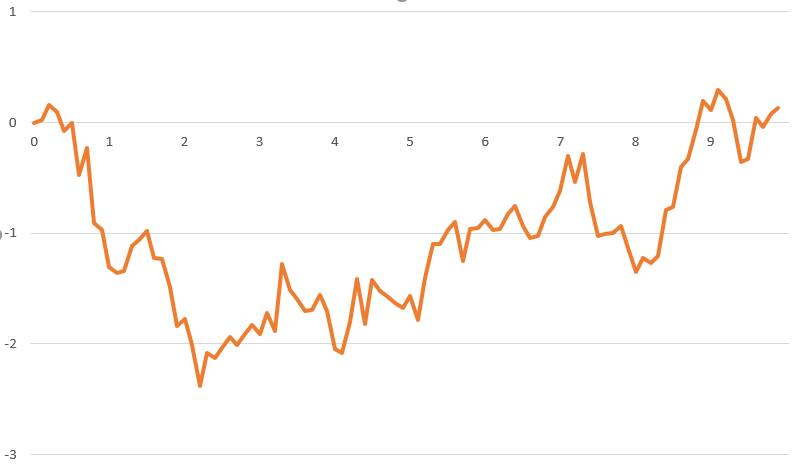
\includegraphics[width=10cm]{brown}
    \caption{Przykładowy jednowymiarowy proces Weinera (ruch Browna)}
    \label{fig:brown}
\end{figure}
Jak możemy zaobserwować na rysunku \ref{fig:brown} pomimo, iż wysokość wykresu ciągle się zmienia, to często wahania te pozostają w granicach przedziału precyzji. A więc wykonanie pomiaru w 6 i 7 sekundzie wyprodukuje identyczny rezultat. Stąd też wymagają czasu, aby temperatura zmieniała się na tyle, żeby nasz system był w stanie wykryć różnicę. Częstym problemem jest również sama ilość próbek, które urządzenie pomiarowe jest w stanie w ciągu sekundy wygenerować urządzenie pomiarowe.
\item[ryzyko manipulowania wynikami:] świat zewnętrzy jest niemożliwy do kontrolowania z punku widzenia twórcy sytemu. Istnieje więc ryzyko, iż osoba posiadająca dostatecznie dużo wiedzy na temat działania pewnego systemu tworzącego liczby losowe będzie w stanie manipulować warunkami środowiskowymi na tyle, żeby wygenerował oczekiwany przez nią rezultat. Możemy np. ciągle ogrzewać czujnik temperatury tak, żeby nigdy nie pokazał, iż temperatura spada lub wręcz sprawić, żeby przekroczył on zakres swoich odczytów.
\item[dostęp do świata zewnętrznego:] w celu pobrania informacji o jakimś parametrze ze świata zewnętrznego konieczny jest czujnik, który jest w stanie odczytać jego wartość. Co oczywiście, nie jest możliwe zmierzenie temperatury bez termometru. W celu generowania odpowiedniej liczby próbek potrzebny jest jednak odpowiedniej klasy sprzęt pomiarowy podnosząc tym samym koszty produkcji urządzenia, który takowy posiada. Stąd tego typu moduły nie są popularne, zwłaszcza w tanich urządzeniach. Pewnym obejściem problemu jest wykorzystanie użytkownika jako źródła entropii dla systemu. Jest to jednak rozwiązanie relatywnie wolne i może być zastosowane jedynie w systemach, w których występuje interakcja z użytkownikiem.
\item[niepewność jednostajności liczb losowych:] oderwanie się od matematycznych wzorów powoduje, iż nie możemy przeprowadzić dowodu poprawności działania takich generatorów. Sprawia to, że nie możemy być pewni parametrów rozkładu naszych zmiennych losowych. Zapewnienie jego jednostajności jest jedną z największych trudności w tym podejściu.
\end{description}

\section{Koncept generatora}
Generator spełniający oba wymagania sprecyzowane w celu tej pracy musi należeć do kategorii ''prawdziwych'' generatorów liczb losowych. Tak więc będzie on wykorzystywać informacje o świecie zewnętrznym celem generowania kolejnych liczb losowych.
\subsection{Źródło entropii}
W tym celu wykorzystamy opóźnienia w przesyłaniu pakietów przez sieć globalną. Jednym powodem ich powstawania na drodze naszego pakietu będzie obciążenie hosta docelowego. Jest on praktycznie zupełnie poza naszą kontrolą i wynika z liczby użytkowników chcących pobrać z niego informacje, a więc jest wypadkową tysięcy niezależnych od nas decyzji ludzkich jak i również zautomatyzowanych systemów. Pomiędzy naszym komputerem, a hostem docelowym występuje pewna liczba komputerów (routerów) odpowiedzialnych za przekierowywanie pakietów do celu. Każdy z tych routerów również generuje opóźnienia wynikające z ich obecnego obciążenia. Tak więc nawet jeśli jako jedyni chcemy sprawdzić ceny akcji firmy \emph{Apple}, to na czas uzyskania tych informacji ma również wpływ sąsiadka wyszukującą w Internecie filmiki z kotami. Ostatnim z źródeł opóźnień na drodze pakietu jest czas jego przetworzenia przez nasz komputer co więcej, że warunki środowiskowe takie jak temperatura powietrza, opady atmosferyczne czy nawet promieniowanie kosmiczne na trasie pakietu mają również pewien, choć bardzo niewielki wpływ na jego czas podróży.  
\subsection{Przekształcenie próbek na liczby losowe}
Posiadając już odpowiednio losowe źródło entropii, którym dla naszego przypadku będzie dodatnia liczba naturalna określająca czas podróży pakietu w pewnej jednostce czasu, należy je jeszcze odpowiednio przetworzyć, aby zapewnić oczekiwany jednostajny rozkład liczb losowych. W przypadku tej pracy, w tym celu ''obetniemy'' każdą próbkę do najmniej znaczących bitów, używając w tym celu operacji modulo. Część z bitów naszej próbki powinna mieć rozkład statystycznie nieróżniący się od rozkładu jednostajnego.

\section{Występowanie prawa Benforda w rozkładzie czasów dostępów}
\subsection{Definicja}
Rozkład zmiennej losowej $X$ spełnia prawo Benforda wtedy i tylko wtedy gdy $Lead(X)$ (funkcja zwracająca najbardziej znaczącą cyfrę) spełnia warunek \ref{eq:benford_def}:
\begin{equation}
    \label{eq:benford_def}
    P(\textrm{Lead}(X) = d) = \log_b(d+1)-\log_b(d) = \log_b\left(1+\frac{1}{d}\right)
\end{equation}
gdzie $b$ oznacza podstawę systemu liczbowego w którym zapisana jest dana liczba.
\subsection{Historia}
Pierwszym opublikowanym artykułem na temat tego fenomenu jest \emph{Note on the frequency of use of the different digits in natural numbers} (tłum. \emph{Uwaga na temat częstotliwości występowania różnych cyfr w liczbach naturalnych}) \cite{first_benford}. W nim właśnie Simon Newcomb podzielił się obserwacją, iż najbardziej znaczące cyfry (1-9) nie występują w jednakowej proporcji. Swojego odkrycia dokonał, gdy zauważył że pierwsze strony książki zawierającej wyliczone logarytmy są bardziej  zniszczone niż dalsze. Zaproponował on przedstawioną wyżej formułę opisującą to zjawisko. Kolejnym matematykiem zajmującym się tym problemem był Frank Benford. Na podstawie danych z kilkunastu dostępnych baz danych zauważył on, że około połowa z nich spełnia nazwane od jego nazwiska prawo Benfoda \cite{benford}. Formalizacji tego fenomenu dokonał amerykański matematyk Ted Hill \cite{hill}.
\subsection{Uogólnienie na dalsze cyfry}
Posiadając podaną wyżej definicję prawa Benforda możemy łatwo uogólnić ją na dalsze cyfry. Aby tego dokonać należy zmienić podstawę systemu z $b$ na $b^{k}$ (gdzie $k$ jest $k$-tą najbardziej znaczącą cyfrą). Teraz możemy obliczyć prawdopodobieństwo występowania każdej $k$ cyfrowej kombinacji na początku. Należy jednak pamiętać, że dopuszczalne kombinacje muszą być większe bądź równe $b^{k-1}$, gdyż w przeciwnym wypadku na pierwszej pozycji takiej kombinacji będzie występowało zero, a więc nie będzie to najbardziej znacząca cyfra. Z tych obserwacji możemy wyciągnąć formułę \ref{eq:benford_gen}.
\begin{equation}
\label{eq:benford_gen}
    \begin{split}
        & P(\textrm{Lead}_k(X) = d) = \\
     & = \log_b\left(1+\frac{1}{b^{k-2}+d}\right) + \log_b\left(1+\frac{1}{b^{k-2}+b+d}\right) + \dots + \log_b\left(1+\frac{1}{b^{k-1}-b+d}\right) = \\
     & =  \sum_{n=b^{k-2}}^{n=b^{k-1}-1}\log_b\left(1+\frac{1}{b n+d}\right)
    \end{split}
\end{equation}
Jak widzimy, obliczenie prawdopodobieństwa każdej kolejnej z cyfr jest wykładniczo bardziej złożone.
\subsection{Obserwacja}
Zgodnie z naszymi założeniami początkowymi moglibyśmy się spodziewać, że ze względu na ogromną ilość czynników mających wpływ na czas dostępu jego rozkład powinien dążyć do rozkładu normalnego ze względu na centralne twierdzenie graniczne. Problematycznym w tej tezie jest natomiast fakt, iż czas dostępu nie może być ujemny. Tak więc dla wartości oczekiwanej rozkładu $M$, prawdą jest, iż $P(X \in [-M, 0]) < P(X \in [2M, 3M])$. Być może jednak wartości tak oddalone od wartości oczekiwanej i tak są pomijalne w całym rozkładzie. 
\begin{figure}[!htp]
    \centering
    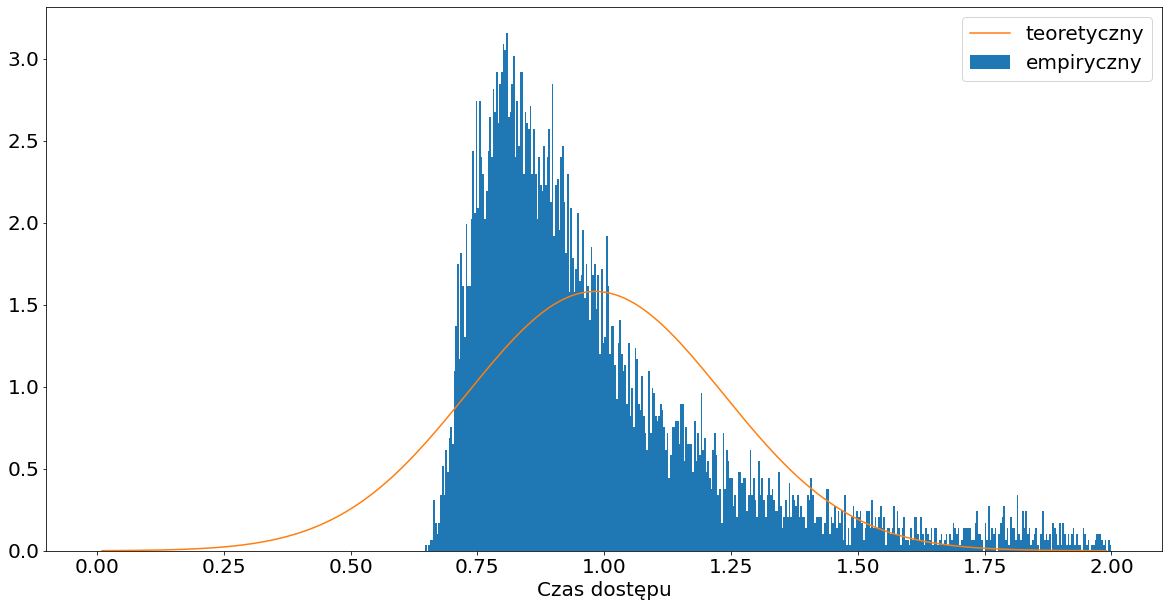
\includegraphics[width=15cm]{norm-ping-dist}
    \caption{Porównanie histogramu czasu dostępu do strony \url{https://www.spaceneedle.com/} z gęstością rozkładu noramlnego}
    \label{fig:bad_dist}
\end{figure}
Jak możemy zobaczyć na rysunku \ref{fig:bad_dist}, rozkład teoretyczny nie pokrywa się empirycznym. Musimy zatem zrewidować swoją tezę. Dokonujemy obserwacji, że $P(X \in [\frac{1}{2}m, m]) \approx P(X \in [m, 2m])$. Możemy zatem postawić hipotezę, iż mamy do czynienia z rozkładem logarytmicznym, precyzyjniej postawimy hipotezę o rozkładzie log normalnym.
\begin{figure}[!htp]
    \centering
    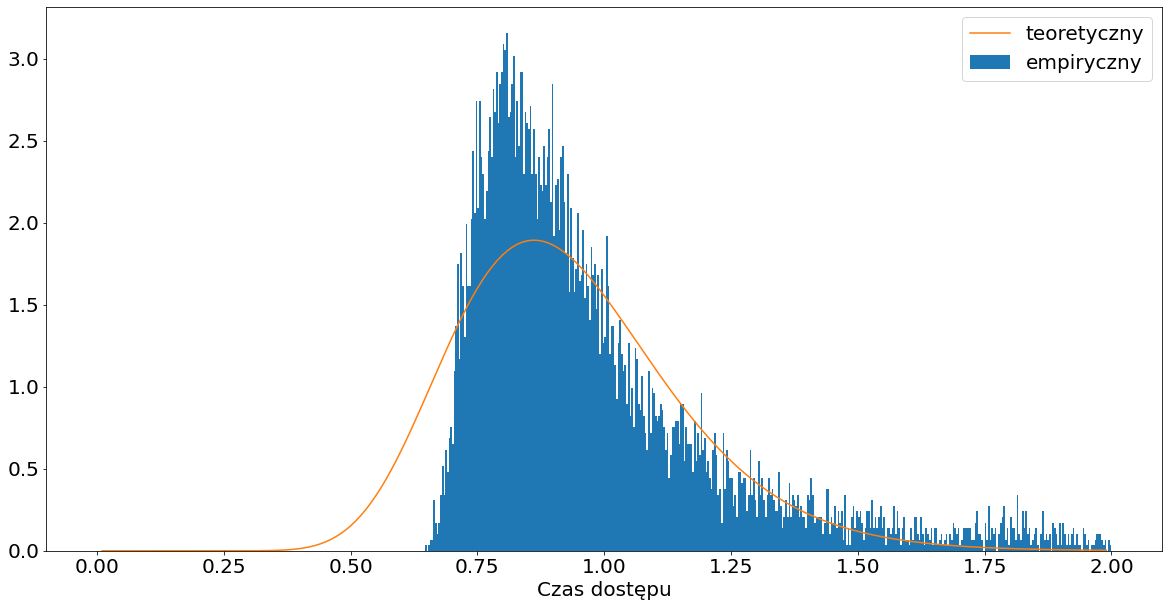
\includegraphics[width=15cm]{lognorm-ping-dist}
    \caption{Porównanie histogramu czasu dostępu do strony \url{https://www.spaceneedle.com/} z gęstością rozkładu log noramlnego}
    \label{fig:better_dist}
\end{figure}
Jak widzimy na wykresie \ref{fig:better_dist} rozkład log normalny lepiej pasuje do empirycznego histogramu. Możemy zatem sprawdzić, czy wygenerowane liczby spełniają prawo Benforda. Jako, iż mamy do czynienia z komputerami, będziemy pracować z systemem liczbowym o podstawie 2.
\begin{table}[H]
\begin{center}

\begin{tabular}{|l|r|}
\hline
Pozycja & \multicolumn{1}{l|}{Prawdopodobieństwo wystąpienia 1} \\\hline
1       & 1                                                    \\\hline
2       & 0.41503749927884376                                  \\\hline
3       & 0.4556794837761896                                   \\\hline
4       & 0.47755858383690225                                   \\\hline
5       & 0.48874172051300435                                   \\\hline
6       & 0.49436607559162077                                  \\\hline
7       & 0.49718243682965746                                 \\\hline
8       & 0.4985911432029018                                  \\\hline
9       & 0.4992955621971009                                   \\\hline
10      & 0.49982388981450276                                   \\\hline
\dots     & \dots                                                  \\\hline
20      & 0.4999996560346523                                   \\\hline
\dots     & \dots                                                  \\\hline
$\infty$& 0.5 \\\hline                                                
\end{tabular}
    
\end{center}
\caption{\label{tab:benford}Rozkład prawdopodobieństwa występowania 1 na pozycji licząc od najbardziej znaczącej}
\end{table}
W tablicy \ref{tab:benford} możemy znaleźć teoretyczne prawdopodobieństwa występowania 1 na $k$-tym najbardziej znaczącym miejscu.
Porównajmy zatem na rysunku \ref{fig:benford_in_real} uzyskane próbki z teoretycznymi prawdopodobieństwami występowania jedynki na $k$-tej najbardziej znaczącej pozycji.
\begin{figure}[!htp]
    \centering
    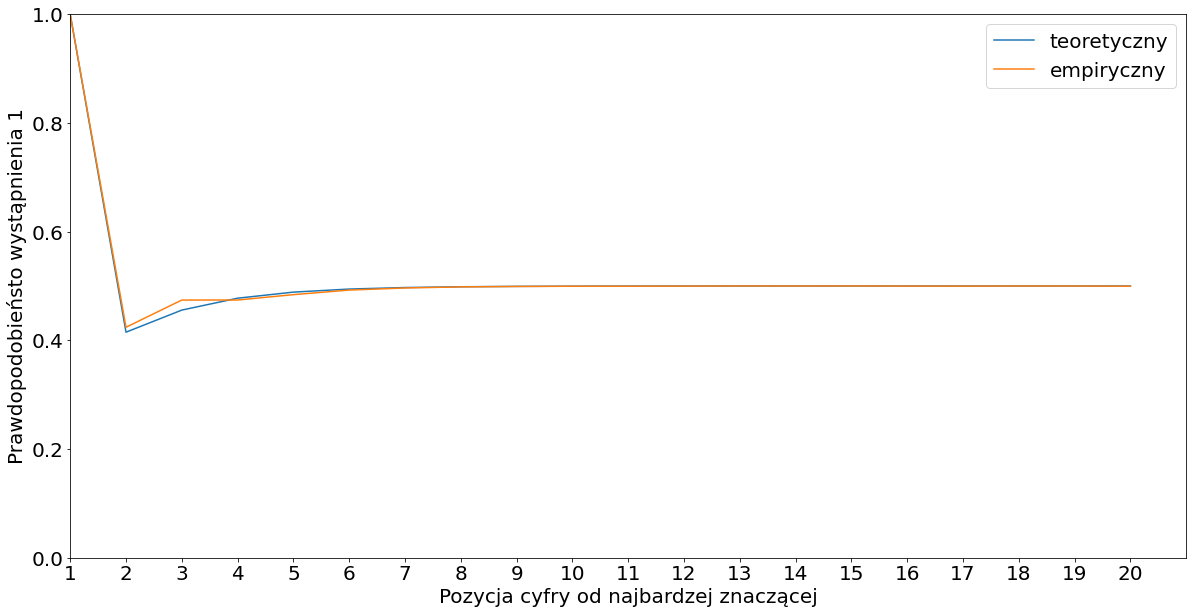
\includegraphics[width=15cm]{benford_comp}
    \caption{Porównanie teoretycznego prawdopodobieństwa występowania '1' na $k$-tej najbardziej znaczącej pozycji (linia niebieska), z empirycznym prawdopodobieństwem (linia pomarańczowa) }
    \label{fig:benford_in_real}
\end{figure}
\subsection{Konsekwencje}
Jak możemy dostrzec na wykresie \ref{fig:benford_in_real}, prawo Benforda dość dobrze opisuje zaobserwowane odchylenie od rozkładu jednostajnego.
Fakt ten rodzi problem przy próbie przekształcenia próbki na ciąg zmiennych losowych o binarnym rozkładzie $(P(X = 0) = \frac{1}{2} \land P(X = 1) = \frac{1}{2})$. Prosta konwersja liczby zmiennoprzecinkowej na ciąg bitów nie zapewni nam oczekiwanego rezkładu. Aby zatem zniwelować ten problem podczas generowania liczb o rozkładzie jednostajnym, wymagane będzie odrzucenie pewnej ilości początkowych bitów, których rozkład będzie najbardziej zaburzony prawem Benforda. Spowoduje to oczywiste obniżenie wydajności generatora w zależności od ilości odrzuconych bitów początkowych z każdej próbki. Konieczne pozostanie zatem balansowanie pomiędzy jednostajnością rozkładu a wydajnością generatora. 
\section{Maksymalna precyzja pomiaru}
\subsection{Jak komputery liczą czas?}
Współczesne komputery posiadają moduł \emph{RTC} (zegar czasu rzeczywistego), który służy jednak głównie do wyświetlania aktualnego czasu, przez co jego precyzja nie jest wystarczająca aby mierzyć czas wykonywania operacji na komputerze. Dlatego też wciąż wykorzystuje się przerwania na procesorze wykonywane co pewną stałą ilość cykli, podczas których następuje inkrementacja licznika czasu. Nie mogą być one jednak zbyt częste, żeby nie obciążać niepotrzebnie maszyny. Oczywiście implementacja tego rozwiązania różni się mocno pomiędzy komputerami, stąd ten sam program może lepiej lub gorzej mierzyć czas w zależności od sprzętu, na którym jest uruchomiony. Dla procesorów o częstotliwości kilku giga Hertzów ($10^9$ operacji na sekundę) precyzyjne odmierzanie upływu nanosekund ($10^{-9}$ części sekundy) zajęłoby większość taktów procesora. Stąd też na takich maszynach możemy spodziewać się jedynie precyzji rzędu mikrosekund ($10^{-6}$ części sekundy). 
\subsection{Wpływ precyzji pomiaru na wydajność}
Precyzja pomiaru w oczywisty sposób wpływa na ilość bitów jakie możemy uzyskać z jednej próbki. Jeśli przymniemy, że uzyskane czasy dostępu będą miały wartości od 16ms do 512ms, to przy precyzji rzędu mikrosekundy możemy uzyskać od 14 do 19 bitów informacji. Zakładając zatem wykorzystanie tylko jednego wątku do tego zadania możemy uzyskać do 875 bitów na sekundę, co jest niewielką wartością, zwłaszcza w porównaniu z generatorami liczb pseudolosowych, które generują kilka kilobajtów danych na sekundę.
\subsection{Konsekwencje}
Taka niewielka ilość bitów uzyskanych z jednej próbki w oczywisty sposób wymusza konieczność zebrania ich większej ilości w celu wygenerowania pojedynczej liczby losowej. Nawet przy  założeniach, że wszystkie bity w tej próbce będą miały oczekiwany przez nas rozkład, przy 16 bitach informacji z każdej, będziemy potrzebować ich aż cztery, aby wygenerować 64 bitową liczbę. Każda próbka generuje obciążenie sieci. Jej przepustowość jest ograniczonym zasobem na każdej maszynie, co jest poważnym problemem w tej metodzie generowania liczb losowych.

	\cleardoublepage

	\chapter{Projekt i implementacja  generatora}
\thispagestyle{chapterBeginStyle}

Rozdział ten jest poświęcony analizie technicznych trudności w implementacji generatora. Dodatkowo zostanie tutaj przedstawiony szczegółowy pseudokod umożliwiający implementację tego rozwiązania w praktycznie każdym języku programowania. Zaprezentowana zastanie również faktyczna implementacja w języku Python oraz analiza wydajności systemu.

\section{Przekształcenie próbki na wektor bitów o jednostajnym rozkładzie}
\subsection{Sposób wyboru bitów z akceptowalnym rozkładem}
Zakładając prawdziwość tezy, iż czasy dostępu spełniają prawo Benforda niemożliwe jest wygenerowanie ze skończonej liczby próbek jednego bitu losowego o rozkładzie jednostajnym. Stąd też obniżyć będziemy musieli nasze oczekiwania odnośnie rozkładu bitów. Zastosujemy prosty test statystyczny, który ocenia szansę uzyskania danej średniej z $n$ próbek zakładając że pochodzą one z jednostajnego rozkładu bitowego. Przyjmiemy standardowy poziom istotności $\alpha = 0.05$, co oznacza, że w 95\% przypadków ciąg bitów z docelowym rozkładem powinien go przejść.
\subsection{Zastosowanie centralnego twierdzenia granicznego}
Dla dużej liczby próbek $X_{i \in \{1, 2, \dots, n\}}$ obliczenie dokładnego rozkładu zmiennej losowej $Y_k = \frac{1}{k}\sum_{i = 1}^{n}X_i$ jest bardzo trudnym zadaniem. Dlatego też zastosujemy centralne twierdzenie graniczne. Mówi one, że dla rozkładu zmiennej losowej $X$, o skończonej wariancji:
\begin{equation}
\begin{split}
\lim_{n \to \infty}\frac{\sqrt{n}}{\sigma n }\sum_{i = 1}^{n}(X_i-\mu) &\sim \mathcal{N}(0, 1)\\
\lim_{n \to \infty}\frac{\sqrt{n}}{\sigma n}\sum_{i = 1}^{n}(X_i) &\sim \mathcal{N}(\mu, 1)\\
\lim_{n \to \infty}\frac{1}{n}\sum_{i = 1}^{n}(X_i) &\sim \mathcal{N}\left(\mu, \frac{\sigma}{\sqrt{n}}\right)\\
\end{split}
\end{equation}
W tej pracy będziemy pracować ze zmienną losową $X \in \{-1, 1\}$ odpowiadającą dwóm stanom bitów:
\begin{equation}
    P(X = 1) = p \land P(X = -1) = 1 - p \label{eq:dist}
\end{equation}
Szybko możemy obliczyć parametry tego rozkładu:
\begin{equation}
\begin{split}
\mathbb{E}X &= 1p+(-1)(1-p) = 2p - 1\\
Var(X) &= \mathbb{E}X^2 - [\mathbb{E}X]^2 = p + (1-p) - (2p-1)^2 \\
&= 1 - 4p^2 + 4p -1 = 4p(1-p)\\
\sigma &= 2\sqrt{p(1-p)}
\end{split}
\end{equation}
Zatem dla odpowiednio dużego $n$, będziemy przybliżać rozkład $Y_n$ rozkładem normalnym o parametrach:
\begin{equation}
    \label{eq:norm_dist_avg}
    \mathcal{N}\left(2p - 1, \frac{2\sqrt{p(1-p)}}{\sqrt{n}}\right)
\end{equation}
\subsection{Test statystyczny}
Celem określenia, jak bardzo podobny jest rozkład bitu do rozkładu docelowego $(p = \frac{1}{2})$ obliczymy prawdopodobieństwo, iż średni wynik dla n zmiennych losowych z rozkładu będzie się mieścił w przedziale: \begin{align*}
    \left[\frac{1}{\sqrt{n}}\Phi^{-1}(0.025), \frac{1}{\sqrt{n}}\Phi^{-1}(0.975)\right]
\end{align*}
gdzie $\Phi^{-1}$ oznacza funkcję odwrotną do dystrybuanty rozkładu normalnego o średniej 0 i odchyleniu standardowym 1. W tym celu skorzystamy z wzoru:
\begin{equation} \label{dist_def}
    P(X \in (a, b]) = F_X(b) - F_X(a)
\end{equation}
gdzie $F_X$ to dystrybuanta rozkładu zmiennej $X$. Przekształcimy teraz dystrybuantę naszego rozkładu tak, aby zachować kształt rozkładu, ale zmienić wariancję i wartości oczekiwaną:
\begin{equation}
\label{eq:dist_trans}
\begin{split}
P(X \leq y) &= F(y) \\
P(\sigma X \leq \sigma y) &= F(y) \\
P(\sigma X + \mu \leq \sigma y + \mu) &= F(y) \\
P(\sigma X + \mu \leq \sigma y) &= F(y - \mu) \\
P(\sigma X + \mu \leq y) &= F\left(\frac{y - \mu}{\sigma}\right) \\
\end{split}
\end{equation}
Wykorzystując przekształcenie \ref{eq:dist_trans} możemy zapisać dystrybuantę $F_{p, n}$ naszego rozkładu dla ustalonego $p$ i $n$, przybliżając ją za pomocą dystrybuanty rozkładu normalnego $\Phi$:
\begin{equation}
    F_{p, n}(y) \approx \Phi \left(\frac{\sqrt{n}(y - 2p - 1)}{2\sqrt{p(1-p)}}\right)
\end{equation}
Dodatkowo oznaczmy jeszcze granice przedziału ufności: 
\begin{equation}
    L_n = -\frac{1}{\sqrt{n}}\Phi^{-1}(0.025) = \frac{1}{\sqrt{n}}\Phi^{-1}(0.975)
\end{equation}
Korzystając zatem z \ref{dist_def} obliczamy szansę przejścia tego testu statystycznego dla dowolnego $p$:
\begin{equation}
    f_n(p)=P\left(X\in [-L_n, L_n]\right) = F_{p, n}(L_n) - F_{p, n}(-L_n)
\end{equation}
Po zaimplementowaniu tej funkcji, możemy zobaczyć jej wizualizację, przedstawioną na rysunku \ref{fig:vis_1} oraz \ref{fig:vis_2}.
\begin{figure}[!htp]
    \centering
    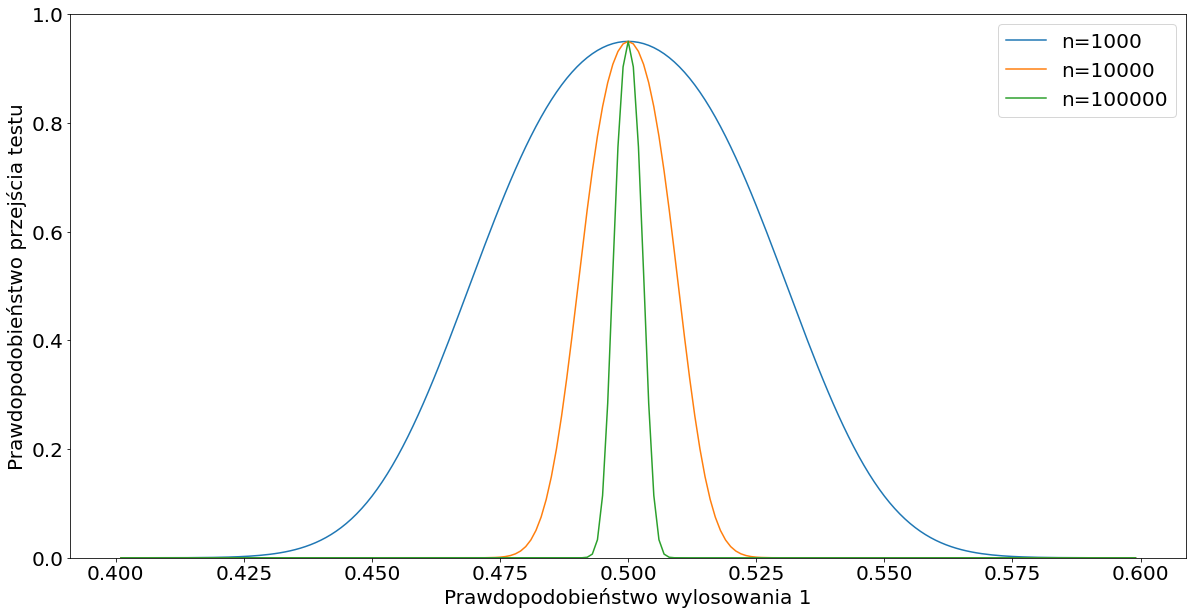
\includegraphics[width=15cm]{chance_of_passing_test_for_n}
    \caption{Porównanie prawdopodobieństwa przejścia testu dla różnych $n$}
    \label{fig:vis_1}
\end{figure}
\begin{figure}[!htp]
    \centering
    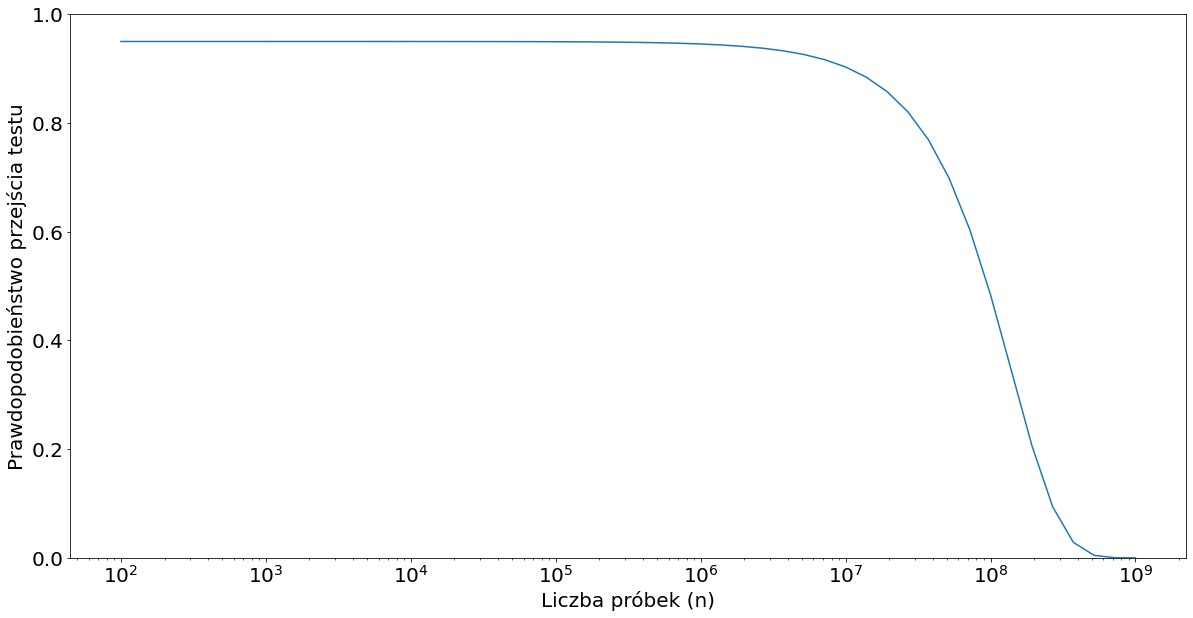
\includegraphics[width=15cm]{probability_of_passing_test_log_scale}
    \caption{Porównanie prawdopodobieństwa przejścia testu dla różnych $n$ (skala logarytmiczna) przy błędzie rozkładu $10^{-3}$}
    \label{fig:vis_2}
\end{figure}
\subsection{Wybranie akceptowalnych rozkładów}
Zakładając prawdziwość tezy o rozkładzie spełniającym prawo Benforda sprawdzimy ile najbardziej znaczących bitów próbki powinniśmy odrzucić. Przyjmijmy za kryterium przejście testu powyżej w 90\% przypadków dla średniej z $10^8$ bitów ($n=10^8$).
\begin{figure}[!htp]
    \centering
    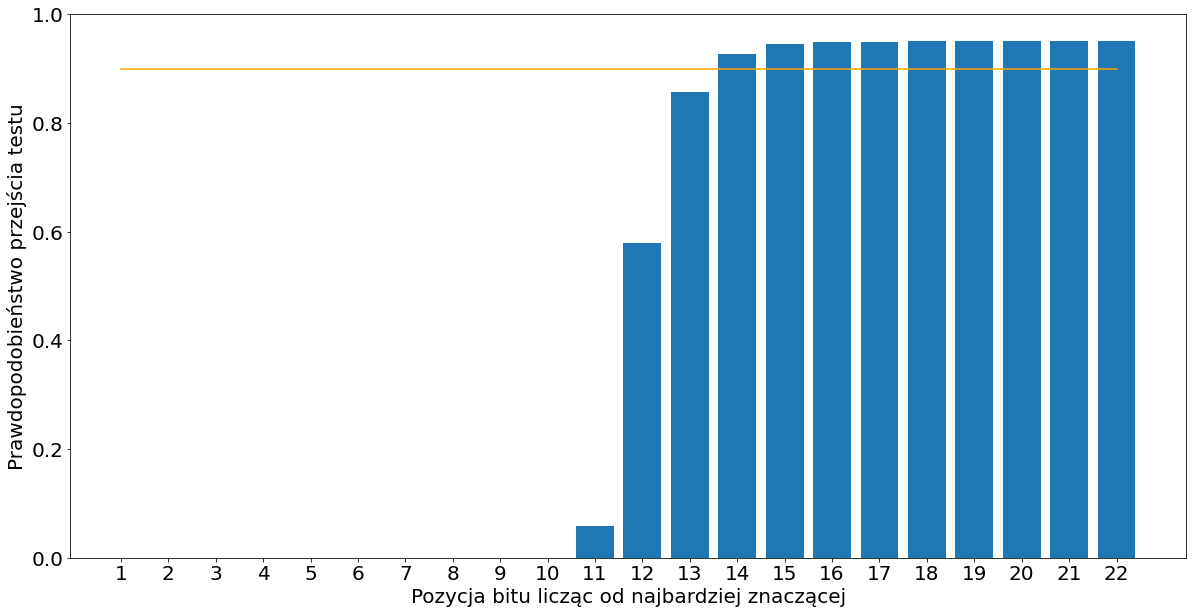
\includegraphics[width=15cm]{probabilty_of_passing_benford}
    \caption{Prawdopodobieństwo przejścia testu statystycznego dla $k$-tego najbardziej znaczącego bitu w próbce spełniającej prawo Benforda (niebieski) oraz próg akceptowalności na poziomie 0.9 (pomarańczowy)}
    \label{fig:probabilty_of_passing_benford}
\end{figure}
Na wykresie \ref{fig:probabilty_of_passing_benford} widzimy, iż bity będące na co najwyżej 14. najbardziej znaczącej pozycji spełniają nasze wymagania. Wcześniejsze niestety będziemy zmuszeni odrzucić ze względu na niekompatybilność rozkładu.
\section{Pseudokod generatora}

{\small
\begin{pseudokod}
\caption{Pseudokod klasy naszego generatora}
\label{alg:gen_code}
\begin{algorithmic}%[1] % uncomment for line numbers
\Class{Generator}
    \State $queue$ : \textsc{SyncQueue<Bit>} \Comment{kolejka synchroniczna bitów}
    \item[]
    \Constructor{$number\_ of\_ threads$ : \textsc{Int}}
        \State $addresses$:\textsc{List<String>} \gets $load()$ \Comment{wczytujemy adresy}
        \For{$i \gets i$ to $number\_of\_threads$}
            \State $thread$ : \textsc{Thread} \gets $Thread$(addresses[i]) \Comment{tworzymy nowy wątek}
            \State $thread$.start() \Comment{uruchamiamy wątek produkujący bity}
        \EndFor
    \EndConstructor
    \item[]
    \Procedure{produce}{$url$ : \textsc{String}}
        \Loop
            \State $time$ : \textsc{Int} \gets $ping$(url) \Comment{pobieramy czas w ns "pinga"}
            \State $bits$ : \textsc{Int} \gets $ceil$($log_2$($time$)) \Comment{obliczamy długość liczby}
            \For{$\_ \gets 14$ to $bits$}
                \State $queue$.push($time$ \textbf{mod} 2) \Comment{dodajemy ostatni bit do kolejki}
                \State $time$ \gets time$ \textbf{div} 2$ \Comment{dzielimy całkowicie przez 2}
            \EndFor
        \EndLoop
    \EndProcedure
    \item[]
    \Function{get}{}
        \State $result$ : \textsc{Int} $\gets 0$
        \For{$\_ \gets 0$ to 63}
            \State $bit$:\textsc{Bit} \gets queue.$pop$() \Comment{pobieramy bit z kolejki}
            \If{$bit$ == 1}
                \State $result$ \gets result $ * 2 + 1$ \Comment{dodajemy 1 na koniec}
            \Else
                \State $result$ \gets result $ * 2$ \Comment{dodajemy 0 na koniec}
            \EndIf
        \EndFor
        \State \Return $result$ \Comment{zwracamy 64-bitową liczbę}
    \EndFunction
\EndClass
\end{algorithmic}
\end{pseudokod}
}
Na podstawie konceptu naszego generatora oraz rozpoznanych potencjalnych problemów możemy przygotować jego pseudokod. Wykorzystamy w nim paradygmat programowania obiektowego, który jest obecnie dostępny w większości najpopularniejszych języków programowania. W pseudokodzie \ref{alg:gen_code} wykorzystamy następujące typy:
\begin{description}
\item[$SyncQueue$] - kolejka synchroniczna. Jest strukturą generyczną, a więc może przechowywać wartości dowolnego określonego typy.  Posiada ona bufor oraz metodę \textbf{$push$} przyjmującą jeden argument, który zostanie dodany do kolejki. W przypadku zapełnienia bufora zatrzymuje wątek do czasu zwolnienia miejsca. Dodatkowo, posiada metodę \textbf{$pop$} która, jeśli bufor nie jest pusty, zdejmuje jeden element z kolejki i go zwraca, a w przypadku pustego bufora zatrzymuje wątek do czasu wprowadzenia do niego danych.
\item[$Thread$] - typ reprezentujący wątek w programie. W konstruktorze przyjmuje funkcję, którą będzie wykonywał po jego uruchomieniu. Wywołanie metody \textbf{$start$} nie zatrzymuje obecnego wątku, a jedynie tworzy nowy. 
\item[$List$] - implementacja listy uporządkowanej.
\item[$Int$] - prosty typ liczbowy 64-bitowy.
\item[$Bit$] - typ liczbowy mogący przyjąć dwie wartości: 0 lub 1.
\item[$String$] - typ przechowujący łańcuch znaków.
\end{description}
Jedynym polem klasy jest $queue$ typu \emph{SyncQueue\textless Bit\textgreater}. Przechowuje ona wygenerowane do tej pory bity, które zostaną wykorzystane w metodzie \emph{get}. Oprócz konstruktora, w którym możemy określić liczbę wykorzystywanych przez nasz generator wątków, mamy dwie metody:
\begin{description}
\item[$produce$] - odpowiada ona za ciągłe pobieranie czasu dostępu do wskazanego w argumencie $url$ adresu, a następnie umieszczanie pozyskanych w ten sposób użytecznych bitów w kolejce $queue$.
\item[$get$] - umożliwia pobieranie liczby losowej z naszego generatora. Bierze ona z kolejki $queue$ 64 bity i tworzy z nich pojedynczą liczbę losową spełniającą założenia tej pracy.
\end{description}

\section{Wybór protokołu do mierzenia czasów połączeń}
Ważnym z punktu widzenia wydajności systemu jest wybór odpowiedniego protokołu sieciowego, który wykorzystamy w naszym generatorze. Nie powinien mieć wpływu na losowość naszych liczb, stąd też możemy koncentrować się na wydajności rozwiązania i wygodzie jego użycia.
\subsection{Przegląd dostępnych rozwiązań}
Przedstawimy tutaj znalezione metody pozyskiwania czasów dostępu do zasobów sieciowych, a mianowicie:
\begin{description}
\item[ping \textit{ICMP} (\textit{Internet Control Message Protocol})] - najbardziej oczywiste podejście do problemu. Jest on obsługiwany przez zdecydowaną większość hostów i powoduje możliwie najmniejsze obciążenie, co pozwala przesłać jednocześnie większą liczbę zapytań z jego wykorzystaniem. Posiada on jednak podstawową wadę - wymaga dodatkowych uprawnień w celu jego wysłania na współczesnych systemach operacyjnych. Oznacza to konieczność uruchamiania programów z tym generatorem z uprawieniami administratora. Ponadto, zupełnie uniemożliwia jego wykorzystanie w niektórych przypadkach, takich jak front-end aplikacji webowych.
\item[\textit{HTTP} (\textit{HyperText Transfer Protocol})] - niezwykle popularny protokół. Wykorzystuje on $TCP$. Z uwagi na to, że wykorzystują go serwisy webowe znalezienie hostów, z którymi można się połączyć nie stanowi żadnego problemu. Ogromną zaletą tego protokołu jest znacząca liczba bibliotek, które go wspierają. Pozwalają one w większości języków pobrać zawartość strony w jednej linijce kodu. Problemem tego podejścia jest natomiast stosunkowo duży rozmiar pakietów, który zależy od wybranego hosta. Dla przykładu kod źródłowy strony \url{http://www.google.com} waży 128 KB, co nie jest relatywnie ogromną wartością, lecz w przypadku konieczności pobrania milionów takich stron mocno obciąża sieć.  
\item[ping \textit{TCP} (\textit{Transmission Control Protocol})] - inne dobre rozwiązanie umożliwiające mierznie czasu potrzebnego na nawiązanie sesji w protokole \emph{TCP}. Naturalnie nie został on zaprojektowany do mierzenia opóźnień, stąd też nie jest tak lekki jak \emph{ICMP}, a więc wywołuje większe obciążenie sieci. Zaletą tego rozwiązania jest brak konieczności posiadania specjalnych uprawnień, przez co możemy go wykorzystać w prawie każdej sytuacji. Wadą jest jednak fakt, iż pingowanie używając tej metody nie jest powszechne. Dlatego też nie zawsze znajdziemy proste w użyciu biblioteki to umożliwiające. Na szczęście, prawie każdy język ma wbudowane wsparcie dla \textit{socketów}. Mając taką bibliotekę wystarczy napisać funkcję nawiązującą połączenie i natychmiast je zrywającą, zmierzyć potrzebny na to czas. Dodatkową wadą jest to, że ciągłe nawiązywanie i zrywanie połączenia nie jest naturalnym zachowaniem w sieci, stąd też po kilku takich próbach, następujących w krótkich odstępach, czas odpowiedzi hosta będzie mocno się wydłużał.
\end{description}
\subsection{Wybór odpowiedniego protokołu}
Jak widzimy, każda z 3 dostępnych opcji niesie z sobą kilka wad, jak i zalet. Na potrzeby tej pracy zastosujemy ostatnie rozwiązanie - tak zwany ping \textit{TCP}. Generator do testów napiszemy w języku Python. Posiada on wsparcie dla tworzenia \textit{socketów}. W przypadku jego implementacji na front-endzie aplikacji webowej, musielibyśmy skorzystać z \textit{web-socketów}. Konieczność nadawania uprawnień administratora dla każdego uruchomienia programu jest w zbyt dużym utrudnieniem dla użytkownika aby zdecydować się na ten wariant z protokołem \textit{ICMP}. Zmiana wybranego protokołu w już zaimplementowanym generatorze nie jest trudna ze względu na jego prostą strukturę. Bez problemu można użyć bibliotek takich jak: \emph{pyping} (dla pingu \textit{ICMP}), \emph{requests} (dla pobierania zawartości stron) oraz \emph{tcping} (dla pinga w oparciu o protokół \textit{TCP}).
\section{Implementacja w języku Python}
Poniżej znajdziemy kod źródłowy \ref{code:source} naszego generatora. Ze względu na jego stosunkowo małą długość pozwolimy sobie omówić go w całości.
\begin{small}
\lstinputlisting[language=Python, caption=Klasa generatora w języku Python, frame=lines, label=code:source, escapechar=#|]{state_of_art.py}
\end{small}
Warto zwrócić uwagę na dwie użyte stałe:
\begin{description}
\item[TIMER\_RESOLUTION\_IN\_NS] - stałą użyta w linijce \ref{line:time_res}. Określa ona rozdzielczość czasu dla funkcji \emph{perf\_counter\_ns}, a więc najmniejsza zmiana, która powoduje zwrócenie innego wyniku. Wpływa ona bezpośrednio na ilość bitów informacji możliwych do uzyskania z pojedynczej próbki.
\item[MOST\_SIGNIFICANT\_BITS\_TO\_REJECT] - stała zastosowana w lilijce \ref{line:bits_reject}. Oznacza ona liczbę najbardziej znaczących bitów z każdej próbki, którą będziemy odrzucać ze względu na występowanie prawa Benforda.
\end{description}
Dodatkowo napisaliśmy funkcje pomocnicze:
\begin{description}
\item[$ping$] -  w linijce \ref{line:ping}. Tworzy ona domyślny \textit{socket}, a następnie łączy się z hostem z argumentu \emph{address} na porcie 80 używanym przez protokół \emph{HTTP}. Po ustanowieniu połączenia go zrywa.
\item[$load\_file$] - w linijce \ref{line:loadfile}. Wczytuje ona kolejne linie z pliku o nazwie pobranej z argumentu \emph{file\_name} i zapisuje je w liście, która jest zwracana na końcu.
\item[$elapsed$] - w linijce \ref{line:elapsed}. Mierzy ona czas potrzebny na wykonanie funkcji przekazanej w argumencie \emph{fn}, a następnie zwraca wynik w jednostce zapewniającej maksymalną ilość informacji o upłyniętym czasie.
\end{description}
Kod zawiera dwie główne klasy:
\begin{description}
    \item[$Pinger$] - którą możemy znaleźć w linijce \ref{line:pinger}. rozszerzającą klasę wątku. Jej głównym zadaniem jest kolejne odpytywanie adresów z argumentu \emph{addresses}, a następne wysyłanie bitów o odpowiednim rozkładzie za pomocą kanału \emph{output}. Dodatkowo w linijce \ref{line:pinger_stop}. znajduje się procedura \emph{stop}, która pozwala zatrzymać wykonywanie wątku.
    \item[$Generator$] - znajduje się w linijce \ref{line:generator}. Jej zadaniem jest generowanie liczb 64-bitowych na podstawie czasów dostępu do zasobów sieciowych. W konstruktorze przyjmuje ona jeden parametr \emph{threads}, który określa ile wątków będzie wykorzystywał generator do pozyskiwania losowych bitów z czasów dostępu do zasobów sieciowych. Dodatkowo konstruktor wczytuje zawartość pliku zawierającego adresy, do których można się połączyć. Funkcja \emph{get}, którą znajdziemy w linijce \ref{line:get}. pobiera bity z kolejki \emph{\_queue}, a następnie tworzy z nich jedną liczbę losową. Klasa zawiera również metodę \emph{stop} w linijce \ref{line:generator_stop}., której zadaniem jest zakończenie pracy generatora oraz wykorzystywanych przez niego wątków. 
\end{description}
\section{Ocena wydajności generatora}
Po zaimplementowaniu generatora możemy dokonać analizy jego wydajności, a więc określić ile losowych bitów będzie w stanie wyprodukować w ciągu sekundy.
\subsection{Ocena wydajności dla pojedynczego wątku}
\sloppy Jak możemy zobaczyć w kodzie w linijce \ref{line:elapsed}. metoda \emph{elapsed} wykorzystuje metodę \emph{time.pref\_counter\_ns}. Według dokumentacji \cite{PythonTimeDoc} dla systemu Windows zapewnia ona rozdzielczość czasu na poziomie 100 nanosekund. Oznacza to, że z każdymi upłyniętymi 100 ns funkcja \emph{time.pref\_counter\_ns} zwróci inny wynik. Dzieląc go przez 100 możemy uzyskać liczbę składającą się z maksymalnej ilości użytecznych bitów. Każdy wątek czeka do czasu otrzymania odpowiedzi z serwera, zatem ilość wykonanych pingów w ciągu sekundy zależy od czasu oczekiwania na odpowiedź. Z drugiej strony im dłuższy czas tym więcej użytecznych bitów otrzymujemy. Zdecydowaliśmy się odrzucać 13 pierwszych bitów ze względu na ich rozkład, a więc próbki poniżej 800 $\mu$s nie niosą żadnej informacji. Na rysunku \ref{fig:generated_bits_in_time} widzimy wydajność pojedynczego wątku dla różnych czasów pinga.
\begin{figure}[!htp]
    \centering
    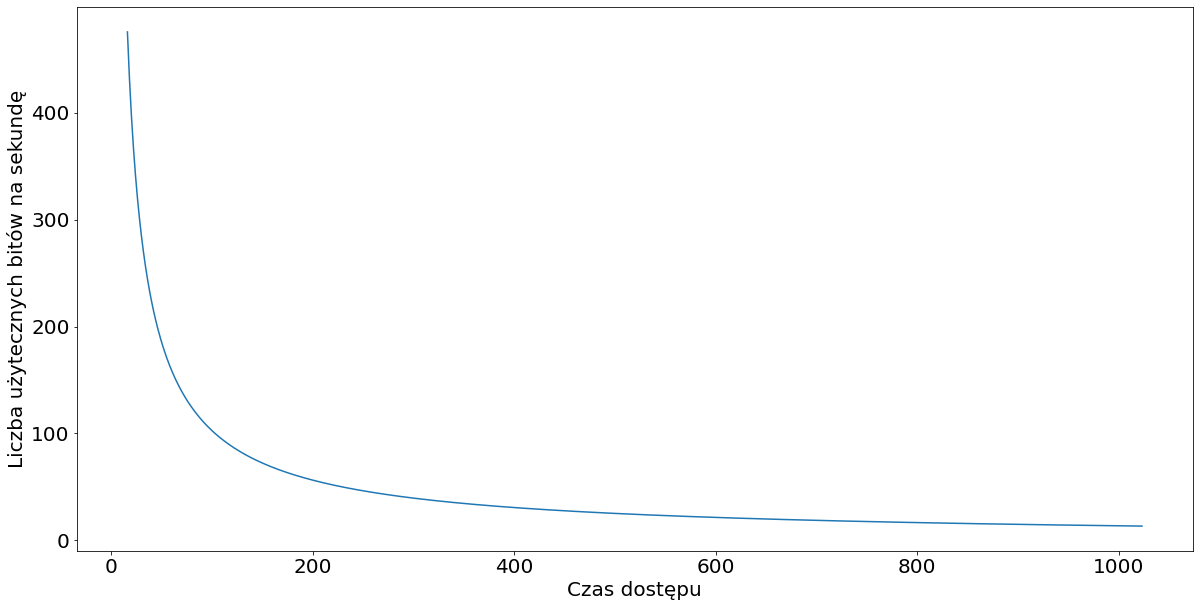
\includegraphics[width=15cm]{generated_bits_in_time}
    \caption{Liczba akceptowalnych bitów uzyskiwanych na jedną milisekundę (oś y), przy stałym czasie pinga w milisekundach (oś x) }
    \label{fig:generated_bits_in_time}
\end{figure}
W praktyce nie udaje się uzyskać czasów lepszych niż 16ms, jeśli chcemy połączyć się do urządzenia spoza naszej sieli lokalnej. W takim przypadku z pojedynczego wątku możemy uzyskać nawet 60 B/s. Jest to relatywnie dobry wynik, choć wypada niezwykle blado w porównaniu z generatorami liczb pseudolosowych. W praktyce jednak średni czas dla pojedynczego pigna w testach wynosił ok. 121 ms. W tym przypadku możemy spodziewać się wydajności rzędu 11 B/s, czyli ok. trzy 64-bitowe liczby losowe na sekundę.  
\subsection{Ograniczenie przez przepustowość sieci}
Aby oszacować jakie obciążenie sieci spowoduje wysłanie jednego pinga \emph{TCP} musimy najpierw zrozumieć jego podstawy. \emph{TCP} jest protokołem połączeniowym, zatem pojedynczy ping wymaga nawiązania połączenia, a następne jego zerwania. 
\begin{figure}[!htp]
    \centering
    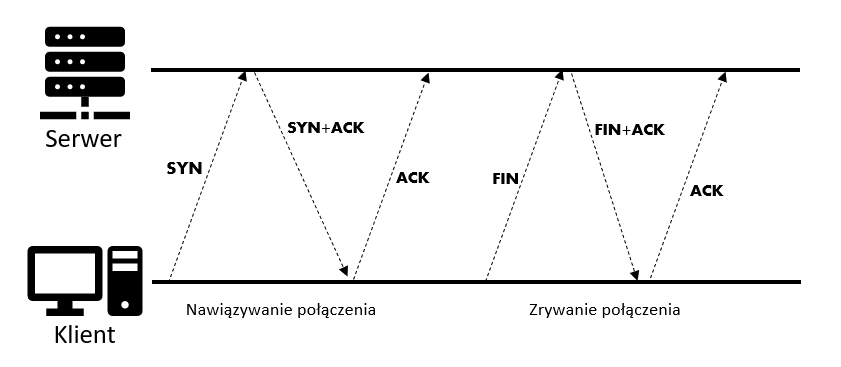
\includegraphics[width=13cm]{tcp_model}
    \caption{Diagram wysyłanych pakietów przy nawiązywaniu i zrywaniu połączenia w protokole TCP}
    \label{fig:tcp_model}
\end{figure}
Jak widzimy na rysunku \ref{fig:tcp_model} ta operacja wymaga wysłania 4 pakietów, przy czym dodatkowo powinniśmy otrzymać 2 pakiety od serwera. Każdy z nich waży od 60 do 80 bajtów. Wykorzystując górne oszacowanie widzimy, że pojedynczy ping wymaga wysłania 320 bajtów oraz pobrania 160 bajtów. Większość dostawców internetu sprzedaje pakiety, których przepustowość wysyłania jest mniejsza od przepustowości pobierania, zatem skupimy się na limicie przepustowości wysyłania. Zakładając, że mamy do dyspozycji łącze o przepustowości wysyłania 1 Mbps, teoretycznie powinniśmy mieć możliwość wykonania 390 pingów na sekundę. Dodatkowym czynnikiem, jaki należy wziąć pod uwagę, jest koszt wykorzystania usługi $DNS$ (\emph{domain name system}). Tłumaczy ona adresy domenowe takie jak \url{www.google.pl} na adresy IP. Jeśli chcemy wykorzystywać adresy w formie domenowej, będziemy umieli do każdego pinga doliczyć ok. 120 bajtów wysłanych oraz 120 bajtów pobranych. Zatem tym samym łączem o przepustowości wysyłania 1 Mbps będziemy teoretycznie mogli wykonać 284 pingów na sekundę.
\subsection{Eksperymentalne wyniki w środowisku testowym}
Znając teoretyczne ograniczenia wydajności naszego generatora warto sprawdzić jak w stosunku do teoretycznych ograniczeń wypada jego wydajność w środowisku testowym. Testy zostały wykonane na prywatnym komputerze w niedzielę o godzinie 18:00. Według serwisu \url{https://www.speedtest.net} wykorzystane połączenie miało 83.75 Mbps przepustowości pobierania oraz 24.29 Mbps przepustowości wysyłania. Zbadaliśmy liczbę pingów na sekundę przy różnej liczbie jednoczesnych pingów. 
\begin{figure}[!htp]
    \centering
    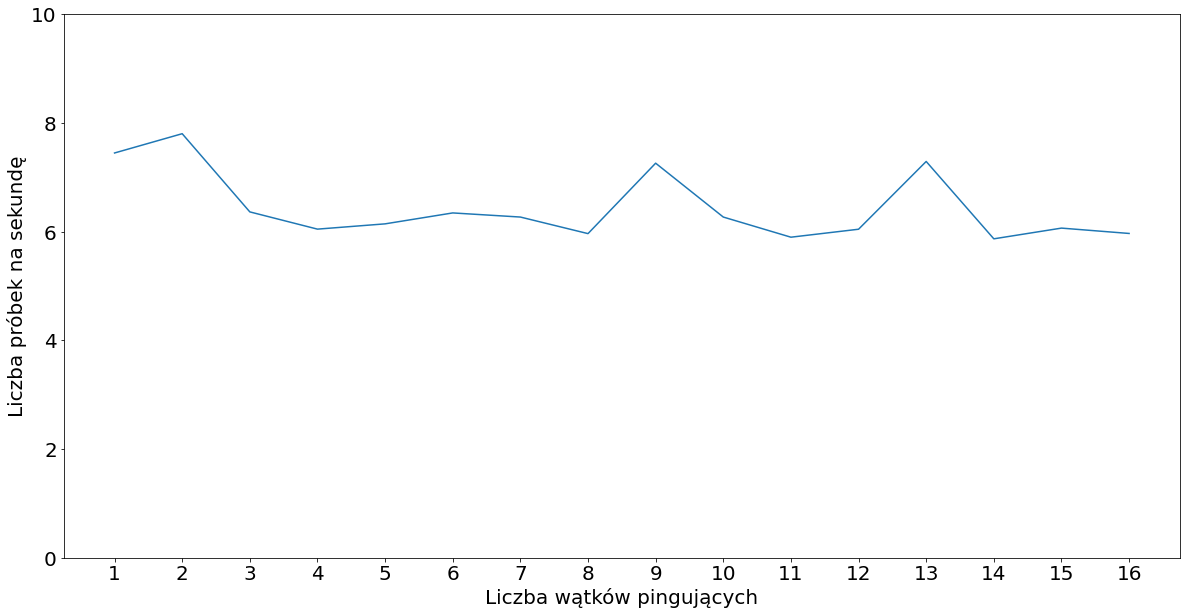
\includegraphics[width=15cm]{performance}
    \caption{Wykres zestawiający liczbę jednoczesnych wątków (oś $x$) z liczbą pingów na sekundę (oś $y$)}
    \label{fig:performance}
\end{figure}
Jak możemy zobaczyć na rysunku \ref{fig:performance}, nie została wykazana żadna istotna korelacja między liczbą wątków a ogólną wydajnością generatora. Spore wahania w wydajności dla różnej liczby wątków zostały prawdopodobnie spowodowane różnicami w obciążeniu sieci w momencie testu. Brak zwiększonej wydajności w przypadku generatora z większą liczbą wątków jest najprawdopodobniej spowodowany limitem ilości przesyłanych pakietów przez lokalny router lub dostawcę internetu. Dalsze badania są wymagane w celu jednoznacznego ustalenia przyczyny problemów z straconymi pakietami w przypadku testów z dużą liczbą jednoczesnych pingów.
	\cleardoublepage
	
	\chapter{Testy losowości}
\thispagestyle{chapterBeginStyle}

Rozdział ten poświęcony będzie testowaniu losowości wyników w celu ustalenia, czy liczby losowe otrzymane z naszego generatora spełniają warunek jednostajności oraz niezależności. Sprawdzimy, jak wypada on w stosunku do znanych rozwiązań. Opiszemy również teorię dotyczącą testowania losowości ciągów bitowych.

\section{Jak udowodnić losowość?}
Krótka odpowiedź brzmi na zadane w tytule niniejszego podrozdziału pytanie mówi, iż nie jest to możliwe. Aby móc powiedzieć z pewnością, jakimi parametrami cechuje się testowany generator, musielibyśmy poznać nieskończoność wygenerowanych przez niego wyników. Załóżmy, że wygenerował on do tej pory ciąg $N$ jedynek. Moglibyśmy rzucić zatem tezę, iż nie spełnia on założenia jednostajności. Wiemy że:
\begin{equation}
\begin{gathered}
    P(X = \mathbb{1}^N) = 2^{-N}\\
    \lim_{N \to \infty} P(X = \mathbb{1}^N) = \lim_{N \to \infty} 2^{-N} = 0
\end{gathered}
\end{equation}
Istnieje zatem szansa, że prawidłowy generator wyprodukuje taki ciąg. Żyjemy w skończonym świecie, a więc empiryczne sprawdzenie granicy dla $N$ dążącego do nieskończoności jest niemożliwe. Co za tym idzie, nie możemy matematycznie udowodnić, iż nie spełnia założeń.
\subsection{Redukcja oczekiwań}
Jesteśmy zmuszeni zatem  zredukować nasze oczekiwania odnośnie testowania generatorów, z matematycznego dowodu, do statystycznego prawdopodobieństwa. Nawiązując do poprzedniego przypadku wiemy, że uzyskanie wektora samych jedynek było zawsze możliwe, jednak szansa na to jest bardzo mała. Uzyskanie dowolnego $n$-elementowego wektora binarnego jest jednakowo prawdopodobne przy założeniu jednostajności i niezależności. Musimy zatem znaleźć jakąś funkcję mierzalną (w naszych zastosowaniach: w sensie Lebesqua), która nie będzie różnowartościowa i zmapuje wiele podobnych wektorów na tę samą wartość. Dobrym przykładem  będzie tutaj  np. stosunek zer do wszystkich cyfr. Jak nietrudno policzyć, dla generatora spełniającego założenie jednostajności, stosunek ten powinien wynosić $\frac{1}{2}$. Istnieją również tylko dwa najbardziej oddalone od tej wartości wektory: $\mathbb{1}^N$ i $\mathbb{0}^N$. Wiemy więc, że prawidłowy generator ma prawdopodobieństwo wylosowania tak skrajnie rzadko występującego przypadku równe $\frac{1}{2^{n-1}}$.
\section{Teoria testów statystycznych}
Test statystyczny jest to narzędzie pozwalające ocenić prawdopodobieństwo hipotezy statystycznej na podstawie skończonej próbki z pewnej populacji.
\subsection{Hipotezy statystyczne}
Każdy test zaczynamy od sformułowania hipotez:
\begin{description}
\item[hipoteza zerowa ($H_0$)] - podstawowa hipoteza mówiąca o tym, że próbka nie odbiega w żaden statystycznie istotny sposób od przyjętych założeń. W naszym przypadku oznacza to, że próbka została wygenerowana przez generator spełniający założenie jednostajności lub niezależności, albo oba.
\item[hipoteza alternatywna ($H_1$)] – zaprzeczenie hipotezy zerowej. W naszym przypadku hipoteza alternatywna będzie mówiła, że nasza próbka różni się w statystycznie istotny sposób od takich, które wygenerowałby generator spełniający założenie jednostajności lub niezależności, albo oba.
\end{description}

\subsection{Podstawowe definicje}
Wprowadzimy kilka podstawowych pojęć i symboli:
\begin{description}
\item[alfa ($\mathbf{\alpha}$)] - wartość określająca, jaka jest szansa, że generator spełniający hipotezę zerową nie przejdzie testu. Z reguły ustalona na poziomie 5\%.
\item[beta ($\mathbf{\beta}$)] – wartość określająca szansę, że generator spełniający hipotezę alternatywą uzyska pozytywny wynik testu.
\item[przedział ufności] – przedział w którym, zgodnie z rozkładem teoretycznym powinno znaleźć się $1-\alpha$ próbek. Tak jak na rysunku \ref{fig:confidence_interval} powinien on pokrywać najbardziej prawdopodobną część teoretycznego rozkładu. 
\end{description}
W przypadku testów statystycznych bardzo często dokonuje się uproszczenia modelu wykorzystując centralne twierdzenie graniczne zakładając, że populacja ma rozkład normalny. 
Ułatwia to znacząco wyznaczenie zakresów dla przedziałów ufności.
\begin{figure}[!htp]
    \centering
    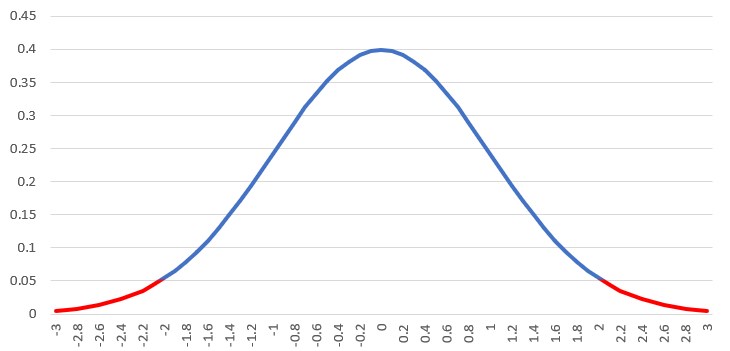
\includegraphics[width=10cm]{confidence_interval}
    \caption{Przedziały ufności(niebieski) dla testu statystycznego z cechą populacji mającą rozkład normalny z $\alpha=0.05$}
    \label{fig:confidence_interval}
\end{figure}
\subsection{Rodzaje błędów}
Przyswoiwszy znaczenie parametrów $\alpha$ i $\beta$ możemy powiedzieć kilka słów o rodzajach błędów, które możemy popełnić w naszym teście.

\begin{table}[!h]
\begin{center}
\begin{tabular}{cccc}
                                            &                          & \multicolumn{2}{c}{Rzeczywistość}                                          \\ \cline{3-4} 
                                            & \multicolumn{1}{c|}{}    & \multicolumn{1}{c|}{H_0}            & \multicolumn{1}{c|}{H_1}             \\ \cline{2-4} 
\multicolumn{1}{c|}{\multirow{2}{*}{Wynik}} & \multicolumn{1}{c|}{H_0} & \multicolumn{1}{c|}{Ok}             & \multicolumn{1}{c|}{Błąd II rodzaju} \\ \cline{2-4} 
\multicolumn{1}{c|}{}                       & \multicolumn{1}{c|}{H_1} & \multicolumn{1}{c|}{Błąd I rodzaju} & \multicolumn{1}{c|}{Ok}              \\ \cline{2-4} 
\end{tabular}
\end{center}
\caption{\label{tab:error_types} Przedstawienie rodzajów błędów w teście statystycznym}
\end{table}
Jak widzimy w tablicy \ref{tab:error_types}, wyróżniamy błąd pierwszego rodzaju (jeśli błędnie odrzucimy hipotezę zerową). Oraz błąd drugiego rodzaju (jeśli przymniemy hipotezę zerową pomimo iż byłą ona fałszywa).
\begin{table}[!h]
\begin{center}
\begin{tabular}{cccc}
                                            &                          & \multicolumn{2}{c}{Rzeczywistość}                                \\ \cline{3-4} 
                                            & \multicolumn{1}{c|}{}    & \multicolumn{1}{c|}{H_0}        & \multicolumn{1}{c|}{H_1}       \\ \cline{2-4} 
\multicolumn{1}{c|}{\multirow{2}{*}{Wynik}} & \multicolumn{1}{c|}{H_0} & \multicolumn{1}{c|}{1 - \alpha} & \multicolumn{1}{c|}{\beta}     \\ \cline{2-4} 
\multicolumn{1}{c|}{}                       & \multicolumn{1}{c|}{H_1} & \multicolumn{1}{c|}{\alpha}     & \multicolumn{1}{c|}{1 - \beta} \\ \cline{2-4} 
\end{tabular}
\end{center}
\caption{\label{tab:error_prob} Przedstawienie prawdopodobieństwa popełnienia błędu w teście statystycznym.}
\end{table}
Z tablicy \ref{tab:error_prob} możemy wyczytać iż $\alpha$ określa prawdopodobieństwo popełnienia błędu pierwszego rodzaju, a $\beta$ prawdopodobieństwo popełnia błędu drugiego rodzaju. O ile z łatwością możemy kontrolować $\alpha$ (wybierając inny przedział ufności, co możemy zobaczyć na rysunku \ref{fig:confidence_interval}), to kontrolowanie, a nawet wyliczenie $\beta$ jest w wielu przypadkach niemożliwe. 
Generatorów produkujących ciągi bitowe jest przynajmniej continuum. Dla każdej liczby rzeczywistej $p \in [0, 1]$ istnieje taki generator, że $(\forall i\in \mathbb{N})P(X_i=1) = p$. Załóżmy, iż mamy do czynienia z niezależnym generatorem o jakimś $p$ oraz, że $p$ zostało wybrane z rozkładem ciągłym. W takiej sytuacji, szansa wybrania $p = \frac{1}{2}$ wynosi dokładnie 0, a więc $\beta = 1$. Takie rozumowanie prowadzi jednak do poważenia zasadności testów statystycznych, przez co nie wyliczamy $\beta$, a jedynie skupiamy się na statystycznie istotnych różnicach.  
Możemy jednak stwierdzić, że dla coraz większej $\alpha$ zmniejsza się $\beta$. W skrajnym przypadku, gdzie $\alpha$ wynosi 1, $\beta$ będzie równa 0. Nie jest to jednak najbardziej użyteczny test, gdyż zawsze odrzuca on hipotezę zerową. Co więcej, o czy, nie należy zapominać, $\beta$ będzie zmniejszać się wraz z zwiększaniem się rozmiaru naszej próbki.
\subsection{Wartość $p$}
Kluczowym pojęciem w testach statystycznych jest wartość $p$ ($P_{\textrm{value}}$). Określa ona, w jakim miejscu teoretycznego rozkładu przy założeniu hipotezy zerowej znajduje się nasza próbka. Im większa wartość $p$, tym większe prawdopodobieństwo, iż została ona wzięta z populacji spełniającej hipotezę zerową, a w naszym przypadku: iż została wygenerowana przez jednostajny i niezależny generator. Obliczenie prawdopodobieństwa tego zdarzenia jak wiemy, jest jednak niezwykle trudne. Otrzymanie skrajnej wartości $p$ nie oznacza, że hipoteza zerowa jest fałszywa; oznacza jedynie, że jest mało prawdopodobna. Co więcej, przy założeniu prawdziwości hipotezy zerowej wartość oczekiwana wartości $p$ to $\frac{1}{2}$, gdyż dla $P_{\textrm{value}}(X) \sim \mathcal{U}(0, 1)$, gdzie $\mathcal{U}(0, 1)$ to rozkład jednostajny na odcinku $(0, 1)$. 
\section{Narzędzia testowania losowości}
Problem określania czy dany wektor bitów jest losowy czy nie, jest relatywnie starym problemem. Od czasów wykorzystywania liczb losowych w kryptografii pojawiło się wiele narzędzi do testowania oraz paczek testów.
\subsection{Przegląd paczek testów losowości}
\begin{description}
    \item[\textit{Ent}] - łatwa w użyciu paczka 5 testów losowości stworzona przez Johna Walkera w 1998 roku. Jest dostępna w dystrybucji Ubuntu. Zawiera dojść prymitywne testy, z których nie każdy posiada wyliczaną wartość $p$. Za pomocą tego narzędzia możemy przetestować wektor losowy dowolnej długości.
    \item[\textit{Diehard}] - pierwotnie wydany na płycie CD w 1995 roku przez George'a Marsaglię zestaw 12 testów na losowość stanowiący, jak na tamte czasy najlepszy tego typu pakiet. Jego użycie jest również proste. Nie zawiera on jednak satysfakcjonującego uzasadnienia matematycznego wykonywanych obliczeń oraz teoretycznego rozkładu, na podstawie którego wyliczane są wartości $p$. Narzędzie możemy znaleźć pod adressem \cite{Diehard}.
    \item[\textit{NIST test suite}] - zestaw 15 testów przygotowanych przez \textit{National Institute of Standards and Technology} w celu sprawdzenia generatorów liczb pseudolosowych do zastosowań kryptograficznych. Używane są jako standard dla kryptografii. Każdy z testów został opisany wa pracy \emph{A statistical test suite for random and pseudorandom number generatorsfor cryptographic applications} \cite{nist}. Zawarte w niej opisy testów nie zawierają sposobu wyliczenia teoretycznego rozkładu. Narzędzie to możemy znaleźć pod adresem \cite{NISTTests}.
    \item[\textit{TestU01}] - najnowsza wersja tej paczki testów pochodzi z 2009 roku, została stworzona przez Pierre L'Ecuyera. Jest ona również powszechnie używana, jednak została przygotowana do testowania generatorów liczb pseudolosowych i wymaga wbudowania swojego generatora w napisany języku w C framework testujący. Narzędzie możemy znaleźć pod adresem \cite{TestU01}.
    \item[\textit{Dieharder}] - narzędzie do testowania losowości stworzone przez Roberta G. Browna. Jego najnowsza wersją powstała w 2020 roku. Paczka zawiera testy z narzędzia \emph{dierhard}, jak również większość przygotowanych przez \emph{NIST} oraz autorskie testy. Jest narzędzie to jest dostępne w dystrybucji Ubuntu oraz pod adresem \cite{Dieharder}. Większość z nich wymaga dużej ilości danych powyżej 100MB. 
\end{description}
\subsection{Wybór generatorów do porównania wyników}
Nasze wyniki porównamy z trzema innymi znanymi generatorami różnej klasy. Przyjrzymy się jak wypada on na tle następujących rozwiązań:
\begin{description}
    \item[\textit{LCG} (\textit{Linear congruential generator})] - jedno z najstarszych i najbardziej znanych podejść do problemu generowania liczb losowych. Logika stojąca za tym generatorem jest łatwa do zrozumienia i sprowadza się do jednego wzoru:
    \begin{equation}
        \label{eq:lcg}
        X_{n+1} = (aX_n + b) \bmod m 
    \end{equation}
    Pomimo swojej prostoty daje on zadowalające wyniki, stąd też jest używany do dziś między innymi w bibliotece \emph{rand} języka C. Do testów użyjemy generatora o parametrach: $m=2^{32}$, $a=22695477$ oraz $b=1$.
    \item[\textit{Tarus}] - rozwiązanie bardzo zbliżone do poprzedniego stworzone przez Pierre L’Ecuyer'a. Posiada bardziej rozbudowany stan wewnętrzny składający się z trzech zmiennych: $s^1$, $s^2$ oraz $s^3$. Zasadę działania generatora opisuje wzór:
    \begin{equation}
        \label{eq:tarus}
        \begin{split}
            X_n &= (s^1_n \oplus s^2_n \oplus s^3_n)\\
            s^1_{n+1} &= ((s^1_n \mathbin{\&} 4294967294) \ll 12) \oplus (((s^1_n \ll 13) \oplus s^1_n) \gg 19)\\
            s^2_{n+1} &= ((s^2_n \mathbin{\&} 4294967288) \ll 4) \oplus (((s^2_n \ll 2) \oplus s^2_n) \gg 25)\\
            s^3_{n+1} &= ((s^3_n \mathbin{\&} 4294967280) \ll 17) \oplus (((s^3_n \ll 3) \oplus s^3_n) \gg 11)
        \end{split}
    \end{equation}
    gdzie $\mathbin{\&}$ oznacza operator iloczynu bitowego (\emph{and}), $\oplus$ oznacza bitową sumę rozłączną (\emph{xor}), a $\ll$ oraz $\gg$ oznaczają operację przesunięcia bitowego, odpowiednio w lewo i prawo.
    \item[\textit{CRNG} (\textit{Cryptographic random number generator})] - generator liczb losowych do zastosowań kryptograficznych. W tej pracy używamy rozwiązania z pakietu \emph{secrets} z języka Python. Wykorzystuje on zebraną przez system operacyjny entropię w celu wygenerowania liczb ''prawdziwie'' losowych.  
\end{description}
\section{Testy losowości}
Ze względu na niezwykle ubogie matematyczne uzasadnienie poprawności testów w znalezionych gotowych narzędziach testujących, jak również ich przystosowanie do testowania generatorów liczb pseudolosowych, wykorzystamy w tej pracy własne testy. Będą on mocno inspirowane pracą \emph{NITS} \cite{nist} wzbogacone o odpowiednie uzasadnienie matematyczne.
\subsection{Test częstotliwości}
\subsubsection{Cel testu}
Ten test skupia się na sprawdzeniu, czy wektor bitów $X$ ma rozkład jednostajny, a więc czy stosunek zer do jedynek dąży do równej proporcji. Jest to jeden z prostszych testów. Polega on na wyliczeniu wspominanej proporcji, a następnie obliczeniu szansy jej otrzymania przy założeniu jednostajności generatora. 
\subsubsection{Matematyczne podstawy testu}
Pierwszym krokiem będzie różnowartościowe zmapowanie wektora $X$ na zbiór $\{-1, 1\}$, tworząc zmienną losową $Y_i = 2X_i - 1$. Jest ona specjalnym przypadkiem rozkładu \ref{eq:dist}, z $p$ równym $\frac{1}{2}$. Korzystając z centralnego twierdzenia granicznego możemy użyć aproksymacji \ref{eq:norm_dist_avg} w postaci:
\begin{equation}
    \mathcal{N}\left(0, \frac{1}{\sqrt{n}}\right)
\end{equation}
Oznaczmy sumę po wszystkich wartościach $Y_i$ jako $S$:
\begin{equation}
    S =\sum_{i=1}^{n}(2X_i-1) = \sum_{i=1}^{n}Y_i
\end{equation}
Oznaczmy dodatkowo $\Phi$ jako dystrybuantę standardowego rozkładu normalnego:
\begin{equation}
    \Phi(x) = \int_{-\infty}^x\frac{1}{\sqrt{2\pi}}e^{-\frac{t^2}{2}} dt = \frac{1}{2}\left(1+ \textrm{erf}\left(\frac{x}{\sqrt{2}}\right)\right)
\end{equation}
gdzie, \emph{erf} jest funkcją błędu Gaussa, zdefiniowaną jako:
\begin{equation}
    \textrm{erf}(z) = \frac{1}{\sqrt{\pi}}\int_{0}^ze^{-t^2} dt
\end{equation}
Z centralnego twierdzenia granicznego wiemy, że w granicy, przy $n \to \infty$:
\begin{equation}
\begin{split}
    \label{eq:bin_norm}
    \frac{S}{n} &\sim \mathcal{N}\left(0, \frac{1}{\sqrt{n}}\right)\\
    \frac{S\sqrt{n}}{n} &\sim \mathcal{N}\left(0, 1\right)\\
    \frac{S}{\sqrt{n}} &\sim \mathcal{N}\left(0, 1\right)
\end{split}
\end{equation}
Możemy zatem, przy $n \to \infty$, skorzystać z dystrybuanty rozkładu normalnego jako dystrybuanty $\frac{S}{\sqrt{n}}$:
\begin{equation}
    \Phi(x) = P(\frac{S}{\sqrt{n}} \leq x) = \frac{1}{2}\left(1+ \textrm{erf}\left(\frac{x}{\sqrt{2n}}\right)\right)
\end{equation}
Standardowy rozkład normalny jest symetryczny ($\Phi(x) = 1-\Phi(-x)$). Możemy uprościć nieco formułę używając wartości bezwzględnej: 
\begin{equation}
\begin{gathered}
    P\left(\frac{|S|}{\sqrt{n}} \geq x\right) = P\left(\frac{S}{\sqrt{n}} \geq x\right) + P\left(\frac{S}{\sqrt{n}} \leq -x\right) =
    1 - P\left(\frac{S}{\sqrt{n}} \leq x\right) + P\left(\frac{S}{\sqrt{n}} \leq -x\right) =\\=
    1 - \Phi(x) + \Phi(-x) =  1 - \Phi(x) + (1 - \Phi(x))  = 2 - 2\Phi(x) = 2\Phi(-x)
\end{gathered}
\end{equation}
Znamy zatem przybliżony teoretyczny rozkład zmiennej $\frac{|S|}{\sqrt{n}}$.
\subsubsection{Wartość $p$}
Dla wektora $X_{i \in \{1, \dots, n\}}$, który przyjmuje wartości 0 lub 1 wartość $p$ wynosi:
\begin{equation}
    P_{\textrm{value}} = 1 - \textrm{erf}\left(\frac{|\sum_{i = 1}^nX_i|}{\sqrt{2n}}\right)
\end{equation}
Przyjmując standardowe $\alpha = 0.05$ jeśli $P_{\textrm{value}} > 0.05$ test uznajemy za zaliczony.
\subsection{Test jedynek w bloku}
\subsubsection{Cel testu}
Test skupia się na ilości występowania jedynek w $M$-bitowych blokach. Zlicza, ile jest bloków o $k$ jedynkach, a następnie ocenia, jak bardzo uzyskany wynik pokrywa się z teoretycznym rozkładem.
\subsubsection{Matematyczne podstawy testu}
Mając $n$ bitów, możemy podzielić je na $N=\left \lfloor{\frac{n}{M}}\right \rfloor$ nienachodzących się na siebie bloków. Każdy z nich może mieć od 0 do $M$ jedynek. Możemy zatem zastosować test $\chi^2$ Petersona. Oznaczmy:
\begin{equation}
    \chi^2 = \sum_{i=0}^M{\frac{(O_i-E_i)^2}{E_i}}
\end{equation}
gdzie:
\begin{description}
    \item[$O_i$] - liczba bloków z $i$ jedynkami,
    \item[$E_i$] - oczekiwana liczba bloków z $i$ jedynkami, która wynosi $N\frac{1}{2^M}{M \choose i}$. 
\end{description}
Dowód testu Petersona o najlepszym dopasowaniu pominiemy w tej pracy. Zainteresowani mogą go znaleźć jednak na stronie \emph{MIT} \cite{Chi_squared}. Przedstawimy jedynie jego zarys, żeby zrozumieć zasadę działania tego testu. Krokiem pierwszym w dowodzie byłoby pokazanie, iż zgodnie z centralnym twierdzeniem granicznym dla każdego $i$ $\frac{(O_i-E_i)^2}{E_i}$ dąży do rozkładu normalnego $\mathbb{Z}_i$. Następny etap to wykazanie, że dowolnie wybrany zbiór $\mathbb{Z}_i$ mocy $M$ będzie niezależny, przy czym ostatnia zmienna będzie oczywiście funkcją pozostałych. Możemy zatem przybliżyć rozkład naszego $\chi^2$ za pomocą rozkładu $\chi^2$ o $M$ stopniach swobody. Dystrybuantę tego rozkładu oznaczmy literą $\Psi$:
\begin{equation}
    \Psi_k(x) = \frac{1}{\Gamma(1/k)}\gamma\left(\frac{k}{2}, \frac{x}{2}\right)
\end{equation}
gdzie:
\begin{equation}
\begin{split}
    \Gamma(z) &= \int_0^\infty t^{z-1}e^{-t}dt\\
    \gamma(z,x) &= \int_0^x t^{z-1}e^{-t}dt
\end{split}
\end{equation}
\subsubsection{Wartość $p$}
Test rozpoczynamy od wyznaczenia wartości $O_i$ dla każdego $i$, a następnie obliczamy wartość $p$:
\begin{equation}
    P_{\textrm{value}} =  1 - \Psi_M\left(\sum_{i=0}^M{\frac{\left(O_i-\frac{N}{2^M}{M \choose i}\right)^2}{\frac{M}{2^N}{M \choose i}}}\right)
\end{equation}
Za pozytywy wynik uznajemy $P_{\textrm{value}} > 0.05$.
\subsection{Test nieprzerwanych ciągów}
\subsubsection{Cel testu}
Skupia się on na liczbie występujących w wektorze, nieprzerwanych ciągach tych samych bitów. Każdy nieprzerwany ciąg zer jest poprzedzony jedynką, nie zawiera żadnej jedynki, a następnym bitem po nim jest jedynka (analogicznie dla ciągu jedynek). Porównamy następnie nasz wynik do teoretycznego rozkładu liczby nieprzerwanych ciągów.
\subsubsection{Matematyczne podstawy testu}
Liczba ciągów zależy bezpośrednio od liczby jedynek ($n_1$) i liczby zer ($n_0$). Przyjętymi przez nas oznaczeniem $n$ będzie $(n_0+n_1)$. Możemy stosunkowo łatwo wyznaczyć rozkład zmiennej losowej ($R$) liczby nieprzerwanych ciągów w $n$-bitowym wektorze:
\begin{equation}
\label{eq:runs_dist}
\begin{split}
    P(R = 2x) &= \frac{2\binom{n_0-1}{x-1}\binom{n_1-1}{x-1}}{\binom{n_0+n_1}{n_1}}\\
    P(R = 2x + 1) &= \frac{\binom{n_0-1}{x}\binom{n_1-1}{x-1} + \binom{n_0-1}{x-1}\binom{n_1-1}{x}}{\binom{n_0+n_1}{n_1}}
\end{split}
\end{equation}
Pierwszym spostrzeżeniem pozwalającym na sporządzenie wzorów \ref{eq:runs_dist} jest fakt, iż każdy ciąg nieprzerwanych jedynek jest przedzielony ciągiem zer, a więc liczba ciągów jedynek nie może się różnić od liczby ciągów zer o więcej niż 1. Tak więc w przypadku parzystej liczby nieprzerwanych ciągów mamy tyle samo nieprzerwanych ciągów zer, jak i jedynek. Przejdźmy zatem do obliczenia, ile wektorów ma dokładnie $x$ nieprzerwanych ciągów. W przypadku parzystej liczby nieprzerwanych ciągów wiemy, że mamy $\frac{x}{2}$ nieprzerwanych ciągów jedynek. Obliczmy więc na ile sposobów możemy podzielić $n_1$ bitów na $\frac{x}{2}$ nieprzerwanych ciągów. Zadanie to jest analogiczne ze znalezieniem $\frac{x}{2} - 1$ początków ciągów, gdyż pierwszy musi zaczynać się od pierwszej jedynki. W takim razie zmuszeni jesteśmy wybrać $\frac{x}{2} - 1$ jedynek spośród $n_1 - 1$, co wynosi oczywiście $\binom{n_1-1}{\frac{x}{2}-1}$. Analogicznie sytuacja wygląda dla zer i nieparzystej liczby nieprzerwanych ciągów.\par
Aby móc zastosować centralne twierdzenie graniczne, pozostaje nam jedynie obliczyć wartość oczekiwaną oraz wariancję. Niestety, pomimo podobieństwa do rozkładu hipergeometrycznego zadanie to nie jest łatwe, gdyż mamy dwa osobne wzory dla liczb parzystych i nieparzystych. Stąd też pominiemy je, wykorzystując wyliczenia zawarte w pracy dostępnej pod adresem \cite{Runs}.
\begin{equation}
\label{eq:runs_E}
    \mathbb{E}R = 2\frac{n_0n_1}{n} + 1
\end{equation}
Pomimo skomplikowania rozkładu wartość oczekiwana z wzoru \ref{eq:runs_E} jest relatywnie prosta. Możemy się pokusić o jej uzasadnienie. Okazuje się bowiem, że z prawdopodobieństwem $\frac{n_0}{n}$ poprzedni bit był zerem, a więc nowy ciąg otrzymamy, jeśli następny będzie jedynką. Mamy na to $\frac{n_1}{n}$ szans, co uzasadnia fragment $\frac{n_0n_1}{n}$. Analogiczne wygląda sytuacja w przeciwnym przypadku, stąd mnożymy człon $\frac{n_0n_1}{n}$ razy 2. Wariancja jest jednak dużo bardziej skomplikowana:
\begin{equation}
\label{eq:runs_Var}
    Var(R) = \frac{2n_0n_1(2n_0n_1 - n)}{n^2(n-1)}
\end{equation}
Dla wzoru \ref{eq:runs_Var} brak niestety łatwych intuicji. Ważną obserwacją jest natomiast symetryczność tego rozkładu.
\subsubsection{Wartość $p$}
Test rozpoczynamy od wyznaczenia liczby bloków 01 i 10 w danym nam losowym wektorze, oznaczenia jej jako $\rho$, oraz obliczenia wartości $n_1$ i $n_0$. Następnie wyliczamy wartość oczekiwaną $\mathbb{E}R$ oraz wariancję $Var(R)$ korzystając z \ref{eq:runs_E} oraz \ref{eq:runs_Var}, po czym wyliczamy wartość $p$:
\begin{equation}
    P_{\textrm{value}} =  1 - \textrm{erf}\left(\frac{|\rho + 1 - \mathbb{E}R|}{\sqrt{2Var(R)}} \right)
\end{equation}
Za pozytywny wynik uznajemy $P_{\textrm{value}} > 0.05$. 
\subsection{Test najdłuższego ciągu w bloku}
\subsubsection{Cel testu}
Skupia się on na wyznaczeniu najdłuższego ciągu jedynek w każdym $M$-bitowym bloku, a następnie ustaleniu, z użyciem testu $\chi^2$ Petersona, jakie jest prawdopodobieństwo, że jednostajny i niezależny generator dał taki rezultat.
\subsubsection{Matematyczne podstawy}
Wyznaczenie prawdopodobieństwa, że losowy wektor $n$-bitowy będzie miał najdłuższy ciąg jedynek długości $k$ jest relatywnie trudnym zadaniem. Zacznijmy od oznaczenia funkcji $A_i(j)$, której wartością będzie liczba wszystkich $j$-bitowych ciągów, a których to długość ciągów jedynek nie przekracza $i$. W oczywisty sposób dla $j \leq i$ $A_i(j) = 2^j$, natomiast w przypadku gdy $j > i$, możemy zaobserwować pewną właściwość. Dla zilustrowania przykładu ustalmy, że $i = 2$, wygenerujemy następujące przedrostki '0', '10' oraz '110' a następnie ''dokljmy'' do nich wektory z ciągami jedynek nie przekraczającymi $i$. Jak możemy zauważyć, każdy ciąg wyprodukowany w ten sposób różni się na którymś bicie przedrostka, a więc nie zliczymy żadnego z nich dwa razy. Możemy zatem sformułować tę właściwość następującym wzorem:
\begin{equation}
    \label{eq:longest_run}
    A_i(j) = \begin{cases}
    \sum_{t=j-i-1}^{j-1}A_i(t) &j > i\\
    0 &j < 0 \\
    2^i &\textrm{w przeciwnym przypadku}
    \end{cases}
\end{equation}
Dokładny dowód możemy znaleźć w artykule Schillinga, umieszczonym w bibliografii \cite{longest_run}. Korzystając ze wzoru \ref{eq:longest_run} możemy wyznaczyć prawdopodobieństwa wytopienia wektora z najdłuższym ciągiem jedynek długości $k$. Niestety metoda ta jest wymagająca obliczeniowo, a wyznaczenie prawdopodobieństw dla bloku rozmiaru $M$ ma złożoność $O(M^2)$. Oznaczmy zatem liczbę bloków z najdłuższym ciąganiem jedynek długości $k$ występującą w wektorze jako $O_k$. Mając wyznaczone prawdopodobieństwa oraz znając wszystkie wartości $O$ możemy znów zastosować test $\chi^2$ Petersona o najlepszym dopasowaniu.
\begin{equation}
    \chi^2 = N\sum_{t=0}^M{\frac{(\frac{O_t}{N}-p_t)^2}{p_t}}
\end{equation}
gdzie:
\begin{description}
    \item[$N$] - liczba bloków, która wynosi $\lfloor \frac{n}{M} \rfloor$,
    \item[$p_t$] - prawdopodobieństwo wytopienia wektora z najdłuższym ciągiem jedynek długości $t$, równe $\frac{A_t(M) - A_{t-1}(M)}{2^M}$.
\end{description}
\subsubsection{Wartość $p$}
Test rozpoczynamy od wyznaczenia wartości $O_t$ oraz $p_t$, dla $t \in \{ 0, \dots, M \}$, po czym następnie obliczamy wartość $p$:
\begin{equation}
    P_{\textrm{value}} =  1 - \Psi_M\left(N\sum_{t=0}^M{\frac{(\frac{O_t}{N}-p_t)^2}{p_t}}\right)
\end{equation}
Za pozytywy wynik uznajemy $P_{\textrm{value}} > 0.05$.
\subsection{Test nieokresowości}
\subsubsection{Cel testu}
Test skupia się na sprawdzeniu czy wektor $t$-bitowy zawiera jakieś zależności cykliczne (np. czy co 5-ty bit ma większe szanse być zerem niż jedynką). Wykorzystamy w tym celu transformatę Fouriera, która pozwala wyróżnić z funkcji okresowej poszczególne występujące w niej częstotliwości, a następnie porównamy otrzymany wynik z teoretycznym rozkładem współczynników transformaty.
\subsubsection{Matematyczne podstawy}
Na początek przypomnijmy, czym jest transformata Fouriera. Dla wektora liczb $X_{n \in \{0, \dots, N-1\}}$ generuje ona następujący wektor liczb zespolonych:
\begin{equation}
    Y_k = \sum_{n = 0}^{N - 1}X_ne^{-\frac{i2\pi}{N}k n} = \sum_{n = 0}^{N - 1}X_n\left(\cos\left(\frac{2\pi}{N}k n\right) + i \sin\left(\frac{2\pi}{N}k n\right)\right)
\end{equation}
\begin{figure}[!htp]
    \centering
    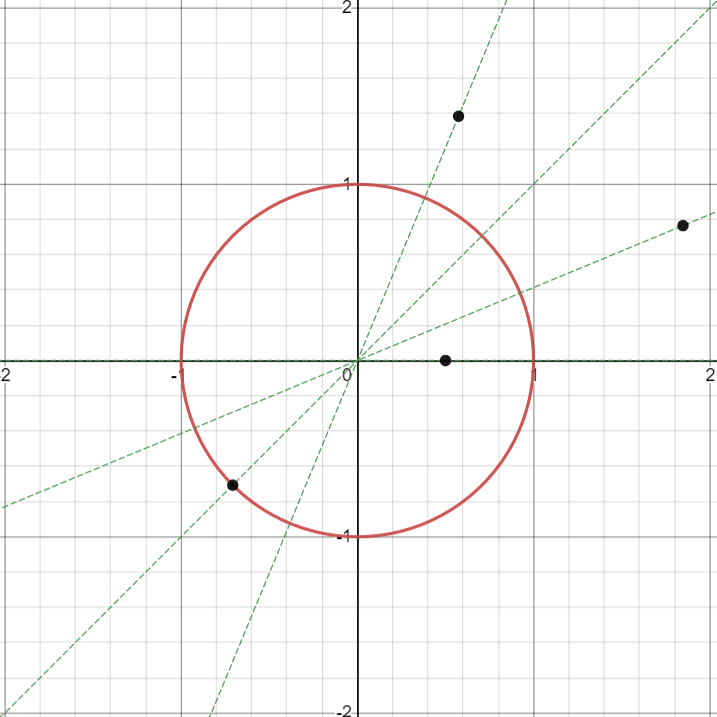
\includegraphics[width=6cm]{furier}
    \caption{Wizualizacja powstawania transformaty Fouriera dla $X=\left[0.5,\ 2,\ -1,\ 1.5,\ \dots\right]$, wykonana w aplikacji Desmos}
    \label{fig:fourier_vis}
\end{figure}
gdzie $i = \sqrt{-1}$. Jej idea opiera się na umieszczeniu punktów wokół początku układu współrzędnych tak, żeby miary kątowe między kolejnymi punktami były identyczne, a odległości od początku układu współrzędnych równe wartościom wektora $X$ (jak możemy zobaczyć na rysunku \ref{fig:fourier_vis}), a następnie obliczeniu średniej pozycji tych punktów. W celu przeprowadzenia testu musimy przyjąć następujące twierdzenia:
\begin{itemize}
    \item Zarówno $\sqrt{\frac{2}{t}} Im(Y_k)$ oraz $\sqrt{\frac{2}{t}} Re(Y_k)$ przy $t \to \infty$ mają rozkład normalny $\mathcal{N}\left(0, 1\right)$,
    \item Zarówno $\sqrt{\frac{2}{t}} Im(Y_k)$ oraz $\sqrt{\frac{2}{t}} Re(Y_k)$ przy $t \to \infty$ są od siebie niezależne,
\end{itemize}
gdzie $Re(z)$ zwraca część rzeczywistą liczby zespolonej, a $Im(x)$ oznacza wartość urojoną liczby. Dowód tych twierdzeń odnaleźć można w pracy \emph{Randomness evaluation with the discrete fourier transform test basedon exact analysis of the reference distribution} \cite{Fourier_test}. Mając te dwa rezultaty możemy w łatwy sposób wywnioskować, iż:
\begin{equation}
    \frac{2}{n}|Y_k|^2 \sim \chi^2_2 \textrm{(rozkład chi kwadrat z 2 stopniami swobody)}
\end{equation}
Znając dokładny rozkład dla $\frac{2}{n}|Y_k|^2$, przy $n \to \infty$ możemy się podjąć się wyznaczenia wartości krytycznej $\kappa$:
\begin{equation}
    \begin{split}
        P(|Y_k| \leq \kappa) &= 0.95\\
        \int_0^{\frac{2}{n}\kappa^2}\frac{1}{2}e^{-\frac{y}{2}}dy &= 0.95\\
        1 - e^{-\frac{\kappa}{n}} &= 0.95\\
        \kappa &= \sqrt{-n\ln{(0.05)}}
    \end{split}
\end{equation}
Ze względu na własność $|Y_k| = |\overline{Y_{N-k}}|$, wykonujemy testy jedynie dla $k \leq \frac{n}{2}$. Ponieważ ten test składa się z $\frac{n}{2}$ testów szansa, że wszystkie z nich przejdą pomyślnie test wynosi $0.95^{\frac{n}{2}}$, co szybko dąży do 0. Dlatego też przy ocenie rezultatu testu musimy pamiętać o tym, iż 5\% z nich powinno uzyskać wynik negatywny. Mamy więc do czynienia z rozkładem Bernuliego.
\begin{equation}
    Z \sim \mathcal{B}(\frac{n}{2}, 0.95)
\end{equation}
Jest to znany rozkład, którego parametry wynoszą:
\begin{equation}
    \begin{split}
        \mathbb{E}Z &= \frac{n}{2}0.95\\
        Var(Z) &= \frac{n}{2}(0.05)(0.95)
    \end{split}
\end{equation}
Możemy zatem korzystając z centralnego twierdzenia granicznego przybliżyć go rozkładem normalnym:
\begin{equation}
    \mathcal{N}\left(\frac{n}{2}0.95, \frac{n}{2}(0.05)(0.95)\right)
\end{equation}
\subsubsection{Wartość $p$}
Celem ustalenia wartości $p$ najpierw dokonamy szybkiej transformaty Fouriera na wektorze bitów zmapowanym funkcją $f(x) = 2x - 1$ (a więc zmieniającą 0 na -1), po czym wyliczamy wektor $r$:
\begin{equation}
    r_k =[\![|Y_k| < \sqrt{-n\ln{(0.05)}}]\!]
\end{equation}
gdzie $[\![$\emph{wyrażenie}$]\!]$ jest funkcją prawdy i przyjmuje 1 (jeśli zdanie jest prawdziwe) i 0 (w przeciwnym wypadku).
\begin{equation}
    P_{\textrm{value}} = 1 - \textrm{erf}\left(\frac{|\sum_{j=0}^{\frac{n}{2}r_k} - \mathbb{E}Z|}{\sqrt{2Var(Z)}} \right)
\end{equation}
Test uznajemy za zaliczony jeśli $P_{\textrm{value}} > 0.05$.
\subsection{Test nakładających się wzorców}
\subsubsection{Cel testu}
Celem testu jest sprawdzenie, czy wstępowanie danego wzorca $B = b_1b_2b_3\dots b_m$ w otrzymanym wektorze pokrywa się z teoretycznym rozkładem przy założeniu jego jednostajności oraz niezależności.
\subsubsection{Matematyczne uzasadnienie}
Obliczenie dokładnego prawdopodobieństwa dla poszczególnej liczby występowania wzorca $B$ w losowym wektorze $X=x_1x_2x_3\dots x_n$ jest bardzo trudnym zadaniem. Możemy poznać dokładne wartości dla wzorców długości 4 \cite{4bits_patterns}, jednak samo wyliczenie wszystkich prawdopodobieństw jest niełatwe ze względu na złożoność obliczeniową. Stąd też użyjemy oszacowania rozkładem normalnym. Żeby to zrobić, musimy najpierw wyznaczyć wartość oczekiwaną oraz wariancję. Aby je obliczyć potrzebujemy nowego wektora zmiennych losowych.
\begin{equation}
    \label{vect_pos}
    Y_k = [\![ x_{k-m+1}x_{k-m+2}\dots x_k = b_1b_2\dots b_m]\!]
\end{equation}
Wektor $Y$ z definicji \ref{vect_pos} informuje nas, czy na $k$-tej pozycji kończy się poszukiwany przez nas wzorzec. Z łatwością możemy obliczyć, że dla każdego $k \in \{m, \dots, n\} Y_k = \frac{1}{2^m}$. Oznaczmy zmienną losową liczbę występowania wzorca $B$ w losowym wektorze jako $Q$. Zatem:
\begin{equation}
    \label{patern_expected}
    \mathbb{E}Q = \mathbb{E}{\sum_{k=m}^n Y_k}=\sum_{k=m}^n \mathbb{E}Y_k = \sum_{k=m}^n \frac{1}{2^m} = \frac{n-m+1}{2^m}
\end{equation}
Wzór \ref{patern_expected} wynika z faktu, iż wartość oczekiwana sumy jest zawsze sumą wartości oczekiwanych, przez co nie musimy przejmować się problemem zależności wektora $Y$. Prawo wariancji sumy jest bardziej skomplikowane:
\begin{equation}
    \label{sum_of_var}
    Var(A+B) = Var(A) + Var(B) + cov(A, B)
\end{equation}
Jak widzimy na wzorze \ref{sum_of_var}, aby policzyć sumę wariancji konieczne jest ustalenie kowariancji zmiennych losowych. Kowariancję definiujemy wzorem \ref{eq:cov_def}.
\begin{equation}
    \label{eq:cov_def}
     cov(A, B) = \mathbb{E}[(A -\mathbb{E}A)(B - \mathbb{E}B)] = \mathbb{E}[AB] - \mathbb{E}A\mathbb{E}B
\end{equation}
Aby wyliczyć wartość wariancji dla $\sum_{k=m}^n Y_k$, zastosujemy proces iteracyjny. Najpierw wyliczymy $Var(Y_m + Y_{m+1})$, następnie $Var((Y_m + Y_{m+1}) + Y_{m+2})$, żeby na samym końcu poznać wartość $Var(\sum_{k=m}^{n-1} Y_k+ Y_{n})$. Musimy być zatem w stanie ustalić wartość wyrażenia \ref{eq:e_sum_x} dla każdego $t$.
\begin{equation}
    \label{eq:e_sum_x}
    \mathbb{E}\left[Y_t\sum_{k=m}^{t-1}Y_k\right] = \mathbb{E}\left[\sum_{k=m}^{t-1}Y_t Y_k\right] = 
    \sum_{k=m}^{t-1}\mathbb{E}\left[Y_t Y_k\right]
\end{equation}
Ponieważ $Y$ jest wektorem zer i jedynek oraz $0x = 0$ możemy wzór \ref{eq:e_sum_x} zapisać w formie wyrażenia \ref{eq:e_sum_x_simpl}, pomijając zbędne zera.
\begin{equation}
    \label{eq:e_sum_x_simpl}
    \sum_{k=m}^{t-1}\mathbb{E}\left[Y_t Y_k\right] =
    \sum_{k=m}^{t-1}\mathbb{E}\left[Y_k | Y_t = 1\right] P(Y_t = 1) = 
    \sum_{k=m}^{t-1}\mathbb{E}\left[Y_k | x_{k-m+1}\dots x_k = b_1\dots b_m \right]P(Y_t = 1)
\end{equation}
Widzimy zatem, iż musimy obliczyć oczekiwaną liczbę wzorców $B$ w wektorze długości $t-1$ znając ostanie $m-1$ pozycji tego wektora. Dla $Y_m, \dots, Y_{t-m}$ wartość oczekiwana się nie zmienia i wynosi $\frac{1}{2^m}$. Dla pozostałych $Y_{t-m+1}, \dots, Y_{t-1}$ natomiast koniecznym będzie wyliczenie wartości, które zależą one od samego wzorca $B$. Kończąc, przemnożymy otrzymaną wartość oczekiwaną przez prawdopodobieństwo, że $Y_t = 1$, a więc przez $\frac{1}{2^m}$.
\subsubsection{Wartość $p$}
Wzorzec $B$ jest nam dany. Pierwszym krokiem będzie wyliczenie jego wartości oczekiwanej $\mathbb{E}Q$, wariancji $Var(Q)$ oraz liczby wystąpień wzorca (do której ustalenia najlepiej zastosować algorytm Knutha-Morrisa-Pratta), oznaczonej $Q$. Podstawiając do wzoru, otrzymujemy:
\begin{equation}
    P_{\textrm{value}} = 1 - \textrm{erf}\left(\frac{|Q - \mathbb{E}Q|}{\sqrt{2Var(Q)}} \right)
\end{equation}
Test uznajemy za zaliczony jeśli $P_{\textrm{value}} > 0.05$.
\subsection{Test złożoności liniowej}
\subsubsection{Cel testu}
W tym teście skupimy się na sprawdzeniu jak dobrze złożoność liniowa $M$-bitowych bloków wektora losowego pokrywa się z oczekiwanymi rezultatami. Złożoność linową zdefiniujemy jako najkrótszy rejestr przesuwający z liniowym sprzężeniem zwrotnym (dalej \emph{LFSR}) który może wygenerować ten ciąg. W celu obliczenia złożoności liniowej bloku wykorzystamy algorytm Berlekampa–Masseya \cite{mass}.
\subsubsection{Matematyczne podstawy testu}
Wyznaczmy teoretyczny rozkład złożoności linowej $\Lambda$ przy założeniu jednostajności i niezależności. Obliczenia zostały oparte na pracy R. A. Rueppela \cite{expected_lfsr}. Dla każdego ciągu $n$-bitów $s^n$ możemy wyliczyć jego złożoność linową $\Lambda(s^n)$. Korzystając z pracy J. Masseya \cite{mass} wiemy, że zachodzi następująca zależność rekurencyjna:
\begin{equation}
\label{eq:req_lfsr}
    \Lambda(s^{n+1}) = \begin{cases} 
    \Lambda(s^n) & \textrm{jeśli najkrótszy LFSR dla $s^n$ produkuje odpowiedni bit}\\
    \Lambda(s^n) & \textrm{jeśli najkrótszy LFSR dla $s^n$ nie jest odpowiedni, ale $ \Lambda(s^n) \geq \frac{n}{2}$}\\
    n -\Lambda(s^n) & \textrm{jeśli najkrótszy LFSR dla $s^n$ nie jest odpowiedni i $ \Lambda(s^n) < \frac{n}{2}$}\\
    \end{cases}
\end{equation}
Oznaczmy teraz liczbę ciągów długości $n$ o złożoności liniowej $L$ jako $N_n(L)$. Ciąg $s^{n+1}$ składa się z ciągu $s^{n}$ z dodanym jednym bitem. Jeśli ten dodatkowy bit odpowiada już istniejącemu najkrótszemu \emph{LFSRowi}, jego złożoność się nie zmienia. Dla przypadku kiedy $\Lambda(s^{n+1}) = L' < \frac{n}{2}$, ponieważ złożoność liniowa nie może spaść po dodaniu bitu, do tej kategorii zaliczymy jednie ciągi $n$ bitów, którym dodano odpowiadający bit, zatem $N_{n+1}(L')= N_{n}(L')$. Ciągi, którym dodano nieodpowiadający bit zmienią swoją złożoność. Dlatego też w przypadku $L' > \frac{n+1}{2}$ liczba takich ciągów wyniesie $N_{n}(n-L')$ (są to te którym wzrosła złożoność) plus $2N_{n}(L')$ (ponieważ dla $ \Lambda(s^n) \geq \frac{n+1}{2}$ złożoność się nie zmienia). W przypadku $L' = \frac{n+1}{2}$ ciągi o długości $n$ z dodanym dowolnym bitem zachowają swoją złożoność, więc $N_{n+1}(L') = 2N_{n}(L')$.
\begin{equation}
\label{eq:num_of_lfsr}
    N_{n+1}(L) = \begin{cases} 
    2N_{n}(L)+N_{n}(n-L) & \textrm{jeśli } L > \frac{n+1}{2}\\
    2N_{n}(L) & \textrm{jeśli } L = \frac{n+1}{2}\\
    N_{n}(L)  & \textrm{jeśli } L < \frac{n+1}{2}\\
    \end{cases}
\end{equation}
Wzór \ref{eq:num_of_lfsr} możemy uprościć do formy \ref{eq:lfsr_simp}, której dowód znaleźć możemy w pracy R. A. Rueppela \cite{expected_lfsr}.
\begin{equation}
\label{eq:lfsr_simp}
    N_{n}(L) = \begin{cases} 
    1 & \textrm{jeśli } n \geq L > 0\\
    2^{\{2n-2L, 2L - 1\}} & \textrm{w przeciwnym przypadku}\\
    \end{cases}
\end{equation}
 Ze względu na dużą dysproporcję w ilości ciągów dla odpowiednich złożoności, zastosujemy grupowanie wyników w $T$-przedziałów o różnej długości dla $M$=1024 ($[0, 255]$, $\dots$, $[510, 511]$, $[512]$, $[513, 514]$, $\dots$, $[786, 1024]$). Zastosujemy zatem test $\chi^2$ Petersona:
\begin{equation}
    \chi^2 = N\sum_{k=0}^{T-1}{\frac{(\frac{O_k}{N}-p_k)^2}{p_k}}
\end{equation}
gdzie:
\begin{description}
    \item[$N$] - liczba $M$-bitowych rozłącznych przedziałów,
    \item[$T$] - liczba kategorii,
    \item[$O_k$] - liczba przedziałów zaliczonych do $k$-tej kategorii,
    \item[$p_k$] - prawdopodobieństwo przynależności do $k$-tej kategorii.
\end{description}
\subsubsection{Wartość $p$}
Test rozpoczynamy od wyznaczania prawdopodobieństwa $p$ dla każdej z kategorii. Następnie dzielimy wektor $X$ na $M$-bitowe bloki. Korzystając z algorytmu Berlekampa–Masseya wyliczamy ich złożoności i dodajemy do odpowiedniej kategorii $O$. Następnie obliczamy wartość $p$:
\begin{equation}
    P_{\textrm{value}} =  1-\Psi_{(T-1)}\left(N\sum_{k=0}^{T-1}{\frac{(\frac{O_k}{N}-p_k)^2}{p_k}}\right)
\end{equation}
Za pozytywy wynik uznajemy $P_{\textrm{value}} > 0.05$.
\subsection{Test ostatniego przecięcia}
\subsubsection{Cel testu}
Test skupia się na sprawdzeniu, kiedy po raz ostatni losowa ścieżka wygenerowana na podstawie wektora losowego $X$ długości $n$ osiągnie wartość zero (innymi słowy kiedy po raz ostatni wyrówna się ilość zer i jedynek w wektorze $X$), a następnie porównaniu tej wartości do teoretycznego rozkładu. 
\subsubsection{Matematyczne podstawy}
Pierwszym krokiem w wyznaczeniu ostatniego punku osiągnięcia 0 będzie zdefiniowanie wektora $Y$, który określa naszą pozycję w kroku $t$:
\begin{equation}
    Y_t = \sum_{k=0}^{t-1}(2X_k-1)
\end{equation}
Naszym celem jest wyznaczenie największego $t$ takiego, że $Y_t = 0$. Dla znanego wektora $X$ obliczenie tej wartości jest prostym zadaniem o złożoności obliczeniowej $O(n)$. Aby przeprowadzić test musimy jednak poznać również teoretyczny rozkład ostatniego przecięcia dla wektorów długości o $n$. Posłużymy się zatem centralnym twierdzeniem granicznym, które pozwoli nam oszacować ten ruch jednowymiarowym ruchem Browna (ściślej: procesem Weinera). Dla takich ruchów możemy zastosować drugie prawo \emph{arcus sinusa}, które brzmi:
\begin{equation}
    \label{eq:arcsin_law}
    P(L \leq x) = \frac{2}{\pi}\arcsin(\sqrt{x})
\end{equation}
gdzie $L$ oznacza ostatni punkt w którym ruch Browna przyjmuje wartość 0. Dowód twierdzenia \ref{eq:arcsin_law} możemy znaleźć w pracy \emph{Arcsine laws and its simulation and application} \cite{arcsin_laws}. Rozkład ten jest dojść płaski, a wartość oczekiwana nie pokrywa się z modą. W związku z tym dla $x \in [0, 1]$ podzielimy wektor $X$ na $N$ 2047-bitowych rozłącznych wektorów. Dodatkowo pogrupujemy wyniki na 16 kategorii, po czym zastosujemy test $\chi^2$ Petersona.
\begin{equation}
    \chi^2 = N\sum_{k=0}^{15}{\frac{(\frac{O_k}{N}-p_k)^2}{p_k}}
\end{equation}
gdzie:
\begin{description}
    \item[$N$] - liczba 2047-bitowych rozłącznych przedziałów, a więc $\lfloor \frac{n}{2047} \rfloor$,
    \item[$O_k$] - liczba przedziałów zaliczonych do $k$-tej kategorii, 
    \item[$p_k$] - prawdopodobieństwo przynależności do $k$-tej kategorii.
\end{description}
\subsubsection{Wartość $p$}
Rozpoczynamy obliczając prawdopodobieństwo dla każdej z kategorii:
\begin{equation}
    p_k = \frac{2}{\pi}\left(\arcsin\left(\sqrt{\frac{128(k+1)}{2048}}\right) - \arcsin\left(\sqrt{\frac{128k}{2048}}\right)\right)
\end{equation}
W kolejnym kroku dzielimy wektor na 2047-bitowe przedziały zliczając, ile wektorów należy do każdej kategorii. Następnie obliczamy wartość $p$:
\begin{equation}
    P_{\textrm{value}} =  1 - \Psi_{15}\left(N\sum_{k=0}^{15}{\frac{(\frac{O_k}{N}-p_k)^2}{p_k}}\right)
\end{equation}
Za pozytywy wynik uznajemy $P_{\textrm{value}} > 0.05$.
\subsection{Test największej sumy}
\subsubsection{Cel testu}
Test skupi się na wyznaczeniu maksymalnej wartości losowej ścieżki wygenerowanej w oparciu o $n$-bitowy wektor losowy $X$, po czym otrzymany wynik zostanie porównana do teoretycznego rozkładu tej zmiennej.
\subsubsection{Matematyczne podstawy}
Na początku przedstawimy kilka użytecznych definicji których użyjemy w dalszym rozumowaniu. Całość jest inspirowana notatkami z wykładu dostępnego pod adresem \cite{Max_Brown}.
\begin{equation}
    \begin{split}
        W_t &= \sum_{k=1}^{t}(2X_k - 1)\\
        T_a &= \min\{t \leq 0: W_t = a\} \\
        M_t &= \max_{0\leq k \leq t}W_k
    \end{split}
\end{equation}
Ze względu na jednostajność rozkładu oraz niezależność, możemy dodatkowo powiedzieć, że: 
\begin{equation}
 \label{eq:dual_brown}
    P(W_t > a | T_a < t) =  P(W_t < a | T_a < t) = \frac{1 - P(W_t = a)}{2}
\end{equation}
Równanie \ref{eq:dual_brown} mówi, że jeśli wiemy, że w jakimś punkcie $T_a$ osiągnęliśmy wartość $a$ to szansa, że jesteśmy poniżej tej wartości jest identyczna jak ta, że jesteśmy powyżej jej. Dodatkowo, z definicji możemy wyczytać, że:
\begin{equation}
\label{eq:m_eq_t}
    (\forall t \in \mathbb{N})(\forall \in \mathbb{N})M_t \geq a \Longleftrightarrow T_a \leq t
\end{equation}
czyli, że jeśli maksimum do punktu $t$ jest większe od $a$ to w którymś punkcie przed $t$ nasz ruch musiał przyjąć wartość $a$.
\begin{equation}
\label{eq:brown_max}
    \begin{gathered}
    P(T_a \leq t) =\\
    =P(T_a \leq t \land W_t>a)+P(T_a \leq t \land W_t<a)+P(T_a \leq t \land W_t=a) = \\
    =2P(T_a \leq t \land W_t>a) + P(T_a \leq t \land W_t=a) =\\
    =2P(M_t \geq a \land W_t>a) + P(W_t=a) =\\ 
    =2P(W_t>a) + P(W_t=a)
    \end{gathered}
\end{equation}
W równaniu \ref{eq:brown_max} sprowadziliśmy problem znalezienia rozkładu największej wartości w naszej ścieżce do znalezienia rozkładu wartości w punkcie $t$. Ma on znany rozkład dwumianowy Bernoulliego. My natomiast przybliżmy go rozkładem normalnym korzystając z centralnego twierdzenia granicznego. Możemy zatem ponownie skorzystać z \ref{eq:bin_norm}.
\begin{equation}
    P(M_t \geq a) = P\left(\frac{M_t}{\sqrt{t}} \geq \frac{a}{\sqrt{t}}\right) = 2P\left(\frac{W_t}{\sqrt{t}} \geq \frac{a}{\sqrt{t}}\right) = 2\left(1 - \Phi\left(\frac{a}{\sqrt{t}}\right)\right)
\end{equation}
\subsubsection{Wartość $p$}
Pierwszym krokiem jest znalezienie największej wartości w losowej ścieżce ($M_n$). Podstawiając ją do wzoru otrzymamy wartość $p$:
\begin{equation}
    P_{\textrm{value}} = 1 - \textrm{erf}\left(\frac{M_n}{\sqrt{2n}}\right)
\end{equation}
Jeśli $P_{\textrm{value}} > 0.05$, to uznajemy test za zaliczony.
\subsection{Test rang macierzy}
\subsubsection{Cel testu}
Celem testu jest sprawdzenie złożoności linowej wektora losowego. W tym celu stworzymy losowe macierze binarne wymiaru $m \times m$, a następnie wyznaczymy ich rangi. Porównamy otrzymane wynik z ich teoretycznym rozkładem dla prawdziwie losowej macierzy.
\subsubsection{Matematyczne podstawy}
Aby przeprowadzić ten test, musimy najpierw wyznaczyć prawdopodobieństwo otrzymania losowej macierzy o wymiarach $m \times m$ z rangą $r$. Zadanie to zaczniemy od wyznaczenia prawdopodobieństwa, iż wektor losowy długości $m$ będzie liniowo zależny od zbioru wektorów o randze $(m - k)$. Wiemy, że dla przestrzeni liniowej o $k$ wymiarach wyznaczonej przez wektory $\mathcal{V} = (v_1, v_2, \dots, v_t)$ możemy znaleźć bazę $\mathcal{U} = (u_1, u_2, \dots, u_k)$, która tworzy identyczną przestrzeń, a wektory są parami rozłączne, co oznacza że jeśli jeden wektor na $t$-tej pozycji posiada jedynkę, to wszystkie pozostałe na $t$-tej pozycji mają zero, formalny zapis w następującej formule:
\begin{equation}
\label{eq:pair_disjoint}
    \begin{gathered}
        u_i = (u_i^1, u_i^2, \dots, u_i^m)\\
        (\forall i, j) u_i^j = 1 \rightarrow (\neg \exists t \not = i) u_i^t = 1
    \end{gathered}
\end{equation}
Aby nowy wektor $q$ był liniowo zależny od bazy $\mathcal{U}$ muszą zachodzić własności \ref{eq:line_dependency_1} oraz \ref{eq:line_dependency_2}:
\begin{equation}
    \label{eq:line_dependency_1}
    (\forall i) q \mathbin{\&} u_i = 0 \lor q \mathbin{\&} u_i = u_i\\
\end{equation}
\begin{equation}
    \label{eq:line_dependency_2}
    (\forall i) q \mathbin{\&} \overline{\left(\sum_{i=1}^{k} u_i \right)} \not= 0
\end{equation}
gdzie $\mathbin{\&}$ oznacza iloczyn bitowy dwóch wektorów, operację sumy dwóch wektorów zdefiniujemy jako ich sumę bitową, a $\overline{a}$ oznacza negację bitową wektora $a$. 
Gdyby nie zachodziła własność \ref{eq:line_dependency_1} (a więc istnieje wektor $u_i$, który pokrywa się jedynie w części z wektorem $q$), to niemożliwym jest stworzenie za pomocą operacji sumy rozłącznej z wektorów bazy $\mathcal{U}$ wektora $q$. Gdybyśmy dodali do sumy rozłącznej wektor $u_i$ nastąpiłoby dodanie bitów, które nie należą do $q$ sumy, natomiast jego nie dodanie spowodowałoby, że część bitów, które powinny być jedynką pozostaną zerem. 
Jeśli natomiast nie zachodziłoby \ref{eq:line_dependency_2} koniecznym byłoby ustawienie bitu, który nie jest jedynką w żadnym wektorze z bazy $\mathcal{U}$, co jest niemożliwe.
Z tych własności możemy wyciągnąć wniosek, iż dla bazy $\mathcal{U}$, istnieje $2^k$ wektorów zależnych, a prawdopodobieństwo wylosowania takiego wektora wynosi $\frac{2^{k}}{2^{n}}$ 
Pozostaje nam zatem wyliczyć prawdopodobieństwo uzyskania macierzy wymiaru $m \times m$ o randze $(m - k)$. Wiemy, iż została zbudowana z $k$ liniowo zależnych oraz $(m-k)$ liniowo niezależnych rzędów. Prawdopodobieństwo otrzymania liniowo niezależnego wektora zależy jedynie od rangi poprzednich wierszy. Niezależnie od ich pozycji stanowią one człon $\prod_{i=0}^{m-k-1}(1-2^{-(m-i)})$. Pozostaje nam jeszcze wyliczenie drugiego członu, a więc prawdopodobieństwo wylosowania $k$ liniowo zależnych wierszy. Niestety, ich pozycja ma wpływ na prawdopodobieństwo, przez co zmuszeni jesteśmy zsumować wszystkie kombinacje. Ostatecznie wzór \ref{eq:prob_of_matrix} wyznacza prawdopodobieństwo uzyskania losowej macierzy $m\times m$ o randze $(m-k)$. Dokładny dowód można znaleźć w książce \emph{Random graphs} \cite{kolchin_1998}. 
\begin{equation}
    \label{eq:prob_of_matrix}
    P_m(k) = 2^{-k^2}\left(\prod_{i=0}^{m-k-1}(1-2^{-(m-i)})\right)\left(\sum_{0\leq i_1\leq\dots i_k\leq m-k}2^{-(i_1+i_2+\dots + i_k)}\right)
\end{equation}
Formuła \ref{eq:prob_of_matrix} jest niestety wymagająca obliczeniowo, w związku z tym wyniki podzielimy na 10 kategorii: $k=0$, $k=1$, $\dots$, $k=8$, $k > 8$, a następnie wykonamy test $\chi^2$ Petersona.
\begin{equation}
    \chi^2 = N\sum_{k=0}^{9}{\frac{(\frac{O_k}{N}-p_k)^2}{p_k}}
\end{equation}
gdzie:
\begin{description}
    \item[$N$] - liczba macierzy $m\times m$,
    \item[$O_k$] - liczba przedziałów zaliczonych do $k$-tej kategorii, 
    \item[$p_k$] - prawdopodobieństwo przynależności do $k$-tej kategorii wyliczone na podstawie wzoru \ref{eq:prob_of_matrix}.
\end{description}
\subsubsection{Wartość $p$}
Pierwszym krokiem jest wyliczenie teoretycznego prawdopodobieństwa dla każdej z dziesięciu kategorii, ustalenie rangi każdej macierzy oraz dodanie jej do odpowiedniej kategorii $O_i$. Następnie wyliczamy wartość $\chi^2$, oraz wartość $p$:
\begin{equation}
    P_{\textrm{value}} =  1 - \Psi_{9}\left(N\sum_{k=0}^{9}{\frac{(\frac{O_k}{N}-p_k)^2}{p_k}}\right)
\end{equation}
Przy wartości $P_{\textrm{value}} > 0.05$ uznajemy test za zaliczony.

\section{Wyniki testów}
Po zapoznaniu się z metodami testowania możemy przeanalizować uzyskane wyniki.
\subsection{Wyniki naszych testów}
Na podstawie przedstawionych powyżej testów stworzyliśmy program sprawdzający losowość w języku Python. Do testów wykorzystaliśmy 12 megabajtowe wektory losowych bitów wygenerowane przez odpowiednie generatory. Test jedynek w bloku oraz test najdłuższego ciągu dla bloków 1024 bitów zostały zmodyfikowane poprzez połączenie mało prawdopodobnych kategorii w jedną większą w celu zminimalizowania błędów numerycznych. Pozostałe testy zostały zaimplementowane bez żadnych zmian.
\begin{table}[!ht]
    \centering
    \begin{tabular}{|l|c|c|c|c|}
    \hline
        \textbf{Nazwa testu} & \textbf{LCM} & \textbf{Tarus} & \textbf{CRNG} & \textbf{Nasz generator} \\ \hline
        Test częstotliwości & 0.12882 & 0.68573 & 0.51296 & 0.11257 \\ \hline
        Test jedynek w bloku (128) & \cellcolor{lred} 0.00000 & 1.00000 & 1.00000 & 1.00000 \\ \hline
        Test jedynek w bloku (1024) & \cellcolor{lred}0.00000 & 0.76419 & 0.86979 & 0.68492 \\ \hline
        Test nieprzerwanych ciągów & 0.65722 & 0.78955 & \cellcolor{lred}0.04002 & 0.58470 \\ \hline
        Test najdłuższego ciągu (64) & \cellcolor{lred}0.00000 & 0.99966 & 0.99996 & 1.00000 \\ \hline
        Test najdłuższego ciągu (1024) & \cellcolor{lred}0.00000 & 0.99826 & 0.69517 & 0.99922 \\ \hline
        Test nieokresowości & \cellcolor{lred}0.00000 & 0.86880 & 0.75849 & 0.27542 \\ \hline
        Test nakładających się wzorców & 0.48773& 0.97426& 0.27960& 0.82126 \\ \hline
        Test złożoności liniowej & 0.99864 & 0.925021 & 0.99146 & 0.99740 \\ \hline
        Test ostatniego przecięcia & \cellcolor{lred}0.00000 & 0.89303 & 0.98706 & 0.83454 \\ \hline
        Test największej sumy & 0.06399 & 0.52433 & 0.71036 & 0.47557 \\ \hline
        Test rang macierzy (32x32) & 0.84882 & 0.92983 & 0.96152 & 0.94216 \\ \hline
        Test rang macierzy (16x16) & 0.85061 & \cellcolor{lred}0.00308 & 0.99792 & 0.97909 \\ \hline
    \end{tabular}
    \caption{\label{tab:my_res}Wyniki naszych testów dla różnych generatorów wuwzględniające wartości $p$ dla poszczególnych testów. Z wyróżnieniem wyniki gdzie wartość $p$ jest mniejsza od poziomu istotności $\alpha = 0.05$}
\end{table}
Jak widzimy w tablicy \ref{tab:my_res} najgorzej poradził sobie generator \emph{LCM}, co jest spodziewane z uwagi na jego prymitywną konstrukcję. Wyniki generatora \emph{Tarus} oraz \emph{CRNG} są bardzo zbliżone, co może dziwić z względu na to, iż generator \emph{CRNG} powinien znacząco lepszej klasy. Najlepiej w testach wypadł nasz generator. Z uwagi, iż testy opierają się na testach statystach nie można wyciągnąć jednak jednostajnych wniosków na temat jego wyższości nad \emph{CRNG}.
\subsection{Wyniki testów narzędziem \textit{Diehard}}
Dodatkowo, wykorzystując narzędzie \emph{Diehard} \cite{Diehard}, przeprowadziliśmy kolejne testy. Dla każdego z nich zwracającego więcej niż jedną wartość $p$, w tablicy \ref{tab:diehard} została zaprezentowana ostatnia z nich.
\begin{table}[!ht]
    \centering
    \begin{tabular}{|l|c|c|c|c|}
    \hline
        \textbf{Nazwa testu} & \textbf{LCM} & \textbf{Tarus} & \textbf{CRNG} & \textbf{Nasz generator} \\ \hline
        Birthday Spacings & \cellcolor{lred}1.00000 & 0.50792 & 0.71394 & 0.03742 \\ \hline
        Overlapping Permutations & 0.82591 & 0.02708 & \cellcolor{lred}0.00131 & 0.54635 \\ \hline
        Ranks of 32x32 matrices & 0.54445 & 0.75272 & 0.65900 & 0.53647 \\ \hline
        Ranks of 6x8 Matrices & \cellcolor{lred}1.00000 & 0.42814 & 0.59030 & 0.32594 \\ \hline
        Monkey Tests on 20-bit Words & \cellcolor{lred}0.00000 & 0.20653 & 0.66948 & 0.89925 \\ \hline
        Monkey Tests DNA & 0.34920 & 0.34380 & 0.86220 & 0.34810 \\ \hline
        Count the 1`s in a Stream of Bytes & \cellcolor{lred}1.00000 & 0.32245 & \cellcolor{lred}0.98657 & 0.48885 \\ \hline
        Count the 1`s in Specific Bytes & 0.74763 & 0.51252 & 0.59320 & 0.52139 \\ \hline
        Parking Lot Test & 0.53309 & \cellcolor{lred}0.02187 & 0.71684 & 0.10980 \\ \hline
        Minimum Distance Test & 0.62647 & \cellcolor{lred}0.00003 & 0.58250 & 0.90770 \\ \hline
        Random Spheres Test & 0.08858 & 0.94746 & 0.43352 & 0.77891 \\ \hline
        The Sqeeze Test & 0.10927 & 0.07114 & 0.35482 & 0.81188 \\ \hline
        Overlapping Sums Test & 0.89813 & 0.15546 & 0.86684 & 0.15546 \\ \hline
        Runs Test & 0.34953 & 0.35924 & 0.55256 & 0.91654 \\ \hline
        The Craps Test & 0.56509 & 0.69635 & 0.08896 & 0.65335 \\ \hline
    \end{tabular}
    \caption{\label{tab:diehard} Wyniki testów narzędziem \emph{Diehard} \cite{Diehard} dla różnych generatorów z uwzględnieniem wartości $p$ dla poszczególnych testów i wyróżnieniem wyników, gdzie wartość p znajduje się poza przedziałem ufności $0.025 < P_\textrm{value} < 0.975$ dla tego narzędzia}
\end{table}
Podobnie jak w przypadku poprzednich testów, tu również nasz generator wypadł najlepiej w porówaniu do wszystkich innych generatorów. Jest on wyraźnie lepszy od rozwiązania \emph{LCM}, jak również wydaje się być lepszy od dwuch pozostałych generatorów.
\subsection{Wyniki testów narzędziem \textit{NIST test suite}}
\begin{table}[!ht]
    \centering
    \begin{tabular}{|l|c|c|c|c|}
    \hline
        \textbf{Nazwa testu} & \textbf{LCM} & \textbf{Tarus} & \textbf{CRNG} & \textbf{Nasz generator} \\ \hline
        Frequency & 0.12233 & 0.91141 & 0.35049 & 0.12233 \\ \hline
        Block Frequency & \cellcolor{lred}0.00000 & 0.53415 & 0.53415 & 0.53415 \\ \hline
        Cumulative Sums & 0.53415 & 0.73992 & 0.35049 & 0.35049 \\ \hline
        Runs & 0.53415 & \cellcolor{lred}0.03517 & 0.35049 & \cellcolor{lred}0.03517 \\ \hline
        Longest Run & 0.21331 & 0.53415 & 0.12233 & 0.53415 \\ \hline
        Rank & 0.73992 & 0.53415 & 0.12233 & 0.53415 \\ \hline
        FFT & \cellcolor{lred}0.00000 & \cellcolor{lred}0.00888 & 0.53415 & 0.35049 \\ \hline
        Non Overlapping Template & \cellcolor{lred}0.03517 & 0.91141 & 0.21331 & 0.35049 \\ \hline
        Overlapping Template & \cellcolor{lred}0.00000 & 0.53415 & 0.06688 & 0.53415 \\ \hline
        Universal & \cellcolor{lred}0.00000 & 0.73992 & 0.73992 & 0.73992 \\ \hline
        Approximate Entropy & \cellcolor{lred}0.00000 & 0.21331 & 0.35049 & 0.73992 \\ \hline
        Serial & \cellcolor{lred}0.00000 & 0.91141 & 0.12233 & \cellcolor{lred}0.00430 \\ \hline
        Linear Complexity & 0.73992 & 0.35049 & 0.06688 & 0.21331 \\ \hline
    \end{tabular}
    \caption{\label{tab:nist}  Wyniki testów narzędziem \emph{NIST test suite}
 \cite{NISTTests} dla różnych generatorów z uwzględnieniem wartości $p$ dla poszczególnych testów i wyróżnieniem wyników, gdzie wartość p jest mniejsza od poziomu istotności $\alpha = 0.05$}
\end{table}
Z względu na przejrzysty interfejs narzędzia \emph{NIST test suite} \cite{NISTTests} przeprowadziliśmy dodatkowe testy z jego wykorzystaniem. Użyliśmy identycznych danych jak w dwóch poprzednich testach, podzielonych na 10 strumieni o długości 10000000 bitów każdy.  Dla spójności zastosowaliśmy poziom istotności $\alpha = 0.05$ (taki jak dla poprzednich testów), pomimo zalecanego $\alpha = 0.01$. W przypadku testów, które narzędzie wykonuje kilkukrotnie w celu poprawienia czytelności w tablicy \ref{tab:nist} zaprezentowano jedynie ostanie wyniki. Możemy w niej zobaczyć, że nasz generator wypada gorzej od generatora \emph{CRNG}. Szczególnie niepokoić może wynik testu \emph{Serial} dla którego wartość p wynosi 0.00430. Oznacza to, iż w jedynie 0.43\% przypadków poprawny generator wygeneruje tak skrajne wyniki. Tak jak w poprzednich testach najgorzej wypada \emph{LCM}. Generator \emph{Tarus} radzi sobie lepiej, jednak również nie przeszedł części testów. \emph{CRNG}, w przeciwieństwie do poprzednich narzędzi, przeszedł wszystkie testy bezbłędnie, jednak w wielu testach wartość $p$ znajdowała się na granicy przedziału ufności.
	\cleardoublepage
	
	\chapter{Podsumowanie}
\thispagestyle{chapterBeginStyle}
Celem pracy było stworzenie konceptu generatora ''prawdziwych'' liczb losowych opartego o entropię pochodzącą z czasów dostępu do zasobów sieciowych oraz zaimplementowanie stworzonego narzędzia w celu wykazania jego poprawności. Wektor liczb będący wynikiem pracy takiego generatora musi spełniać warunek jednostajności oraz niezależności, zatem dodatkowym celem było przygotowanie narzędzi umożliwiających potwierdzenie poprawności rozwiązania poprzez przetestowanie wyników generatora pod tym kątem.\par
Początek pracy omawia czy możliwe jest stworzenie generatora prawdziwych liczb losowych, a który to problem można sprowadzić do pytania na temat determinizmu świata. Kolejna sekcja pochyla się nad analizą dwóch podejść do generowania liczb losowych. Jednym z nich było generowanie liczb na podstawie entropii świata zewnętrznego, natomiast drugim - koncepcja odrzucenia wymogu niezależności na rzecz generowania liczb pseudolosowych. Kolejno zaprezentowany został pomysł na źródło entropii w postaci czasów dostępów do zasobów sieciowych (takich jak czas odpowiedzi na ping) wraz z przesłankami świadczącymi o jego poprawności, po czym przeanalizowano teoretyczne problemy takiego podejścia. Czasy pingów mają specyficzny rozkład, w którym występuje prawo Benforda. Oznacza to, iż prawdopodobieństwo otrzymania jedynki na $k$-tym bicie nie jest stałe i jest zależne od długości liczby. Innym przeanalizowanym problemem była maksymalna precyzja pomiarów czasu, której możemy się spodziewać na współczesnych komputerach oraz jej wpływ na wydajność. Następny rozdział skupiał się na analizie i rozwiązaniu problemów technicznych, które rodził nasz generator. Został w nim omówiony pomysł na niwelowanie skutków niejednostajnego rozkładu bitów poprzez odrzucenie bitów o nazbyt odchylonym rozkładzie. Przedstawiono również kryteria rozkładu bitów akceptowalnych dla naszego generatora oraz zaprezentowano szczegółowy pseudokod generatora wraz z jego implementacją w języku Python i jej omówieniem. Dokonana została  również analiza różnych protokołów sieciowych, które można wykorzystać w celu pozyskania czasów dostępów do zasobów sieciowych. Końcem rozdziału przeprowadzono analizę wydajności już napisanego generatora - zarówno teoretyczną, jak i w środowisku testowym. Ostatni rozdział skupia się na problemie pokazania jednostajności oraz niezależności wektora liczb losowych. Zaczyna się on od wyjaśnienia, dlaczego nie może istnieć matematyczny dowód takich własności, a następnie proponuje testy statystyczne jako alternatywę. Ich idea została dokładanie omówiona uwzględniając problemy jakie rodzą. Następną sekcję poświęcono analizie istniejących już narzędzi testowania losowości oraz wyborze trzech generatorów różnej klasy, z którymi zostanie porównane nasze rozwiązanie. Wyjaśniono następnie, iż gotowe narzędzia nie posiadają satysfakcjonującego uzasadnienia swojej poprawności, przez co przygotowanych 10 testów inspirowanych istniejącymi rozwiązaniami, wzbogaconych o matematyczne uzasadnienie swojej poprawności. Rozdział kończy się zaprezentowaniem wyników przeprowadzonych testów - zarówno tych stworzonych na potrzebę pracy, jak i tych już istniejących.\par
Niniejsza praca wykazała możliwość stworzenia generatora ''prawdziwych'' liczb losowych opartego o czasy dostępów do zasobów sieciowych. Generowany przez niego ciąg liczb spełnia wymogi jednostajności i niezależności nie gorzej niż generatory rekomendowane do zastosowań kryptograficznych. Oznacza to, że teoretycznie nasz generator również mógłby być użyty w miejscach wymagających generowania losowych kluczy bez uszczerbku dla bezpieczeństwa tych systemów. Problemem, którego nie udało się w niniejszej pracy rozwiązać (i który najprawdopodobniej niemożliwy jest do rozwiązania) pozostaje wydajność tego rozwiązania. Spowodowany jest on wykorzystaniem mocno ograniczonego zasobu, jakim jest dostęp do sieci. Z tego powodu, generator ten najpewniej nie znajdzie zastosowania w przemyśle i pozostanie konceptem czystko akademickim. Może on jednak posłużyć jako generator wartości początkowych (seedu) dla generatorów liczb pseudolosowych lub jako dodatkowe źródło entropii dla innych rozwiązań. \par
Dalszych badań wymaga problem znaczącego spadku wydajności w przypadku równoległego pingowana w środowisku testowym. Koniecznym okazuje się także odpowiedź na pytanie, czy problem dotyczy tego jednego środowiska, czy jest szerzej reprodukowany oraz jakie są przyczyny gubienia pakietów, mechanizm wyboru bitów o akceptowanym rozkładzie można by również udoskonalić o użycie bitów o nieakceptowanych rozkładach w celu przekształcenia ich pewnej skończonej ilości w bit o rozkładzie akceptowanym dla naszego generatora, co pozwoliłoby w nieznaczny sposób podnieść wydajność systemu. Innym potencjalnym sposobem na jej podniesienie jest analiza, czy zawartość otrzymywanych pakietów może służyć jako dodatkowe źródło entropii. Z punktu widzenia zastosowań kryptograficznych, najważniejsze jest jednak sprawdzenie, jakie są możliwości manipulowania otrzymanymi czasami dostępów do zasobów sieciowych. Nurtującymi pozostaje pytanie. Czy przeprowadzanie ataku z wykorzystaniem fałszywej bramki domyślnej pozwoliłoby by na manipulowanie wynikami generatora? Czy jednak ze względu na odrzucenie najbardziej znaczących bitów operacja ta jest z praktycznego punktu widzenia niemożliwa do przeprowadzenia?





	\cleardoublepage
	
	
	%%%%%%%%%%%%%%%%%%%%%%%%%%%%%%%%%%%%%%%%%%%%%%%%%%%%%%%%%%%%%%%%%%%%%%%%%%%%%%
	%%%%%%%%%%%%%%%%%%%%%%%%%%%%%%% BIBLIOGRAFIA %%%%%%%%%%%%%%%%%%%%%%%%%%%%%%%%%
	%%%%%%%%%%%%%%%%%%%%%%%%%%%%%%%%%%%%%%%%%%%%%%%%%%%%%%%%%%%%%%%%%%%%%%%%%%%%%%

	\pagestyle{bibliographyStyle}
	\bibliographystyle{plabbrv}
	\selectbiblanguage{polish}
	\bibliography{literatura}
	\thispagestyle{chapterBeginStyle}
        \addcontentsline{toc}{chapter}{Bibliografia}

	\cleardoublepage
	
	%%%%%%%%%%%%%%%%%%%%%%%%%%%%%%%%%%%%%%%%%%%%%%%%%%%%%%%%%%%%%%%%%%%%%%%%%%%%%%
	%%%%%%%%%%%%%%%%%%%%%%%%%%%%%%%%% DODATKI %%%%%%%%%%%%%%%%%%%%%%%%%%%%%%%%%%%%
	%%%%%%%%%%%%%%%%%%%%%%%%%%%%%%%%%%%%%%%%%%%%%%%%%%%%%%%%%%%%%%%%%%%%%%%%%%%%%%
	
	\appendix
	\pagestyle{appendixStyle}
	
	\chapter{Zawartość płyty CD}
\thispagestyle{chapterBeginStyle}
\label{plytaCD}

Dodatek ten krótko omówiona zawartość dołączonej do pracy płyty CD. Zawiera ona implementację generatora jak i testów w języku Python. Umieszczono na niej również wszystkie inne pliki wykorzystane w niniejszej pracy.
\dirtree{%
.1 /.
.2 prepared\_binary.
.3 lcm.bin \DTcomment{binarna postać wyniku pracy generatora LCM}.
.3 tarus.bin \DTcomment{binarna postać wyniku pracy generatora Tarus}.
.3 crng.bin \DTcomment{binarna postać wyniku pracy generatora CRNG}.
.3 my.bin \DTcomment{binarna postać wyniku pracy naszego generatora}.
.2 prepared\_num.
.3 lcm.txt \DTcomment{wynik pracy generatora LCM w postaci 32-bitowych liczb}.
.3 tarus.txt \DTcomment{wynik pracy generatora Tarus w postaci 32-bitowych liczb}.
.3 crng.txt \DTcomment{wynik pracy generatora CRNG w postaci 32-bitowych liczb}.
.3 my.txt \DTcomment{wynik pracy naszego generatora w postaci 32-bitowych liczb}.
.2 tests.
.3 frequency\_test.py \DTcomment{kod testu częstotliwości}.
.3 block\_frequency\_test.py \DTcomment{kod testu jedynek w bloku}.
.3 run\_test.py \DTcomment{kod testu nieprzerwanych ciągów}.
.3 longest\_run\_in\_block\_test.py \DTcomment{kod testu najdłuższego ciągu}.
.3 fourier\_test.py \DTcomment{kod testu nieokresowości}.
.3 overlapping\_template\_test.py \DTcomment{kod testu nakładających się wzorców}.
.3 linear\_complexity\_test.py \DTcomment{kod testu złożoności liniowej}.
.3 last\_cross\_test.py \DTcomment{kod testu ostatniego przecięcia}.
.3 max\_cumsum\_test.py \DTcomment{kod testu największej sumy}.
.3 matrix\_rank\_test.py \DTcomment{kod testu rang macierzy}.
.3 utils.py \DTcomment{kod metod pomocniczych}.
.3 \_\_init\_\_.py \DTcomment{kod modułu tests}.
.2 addresses.txt \DTcomment{lista najpopularniejszych stron www}.
.2 preprocesor.py \DTcomment{funkcje pomocnicze do zapisu lub odczytu danych z pliku}.
.2 generator.py \DTcomment{kod zaprezentowanego generatora}.
.2 test\_generators.py \DTcomment{kod generatorów LCM, Tarus i CRNG}.
.2 testing.py \DTcomment{kod programu testującego}.
}

	\cleardoublepage

\end{document}

